\documentclass[conference]{IEEEtran}
\IEEEoverridecommandlockouts
% The preceding line is only needed to identify funding in the first footnote. If that is unneeded, please comment it out.
\usepackage{cite}
\usepackage{amsmath,amssymb,amsfonts}
\usepackage{algorithmic}
\usepackage{graphicx}
\usepackage{textcomp}
\usepackage{xcolor}
\usepackage{booktabs}
\usepackage{multirow}
\usepackage{array}
\usepackage{url}
\usepackage{subcaption}
\usepackage{microtype}

\def\BibTeX{{\rm B\kern-.05em{\sc i\kern-.025em b}\kern-.08em
    T\kern-.1667em\lower.7ex\hbox{E}\kern-.125emX}}

\begin{document}

\title{SynCura: A Level-3 Multi-Scale Hybrid Deep Learning System for Real-Time Predictive ICU Monitoring with Dual Explainability and Multi-Tier Alerting\\
\thanks{This research prototype was developed in the Department of Computer Science and Engineering at P.~A. College of Engineering, Mangalore, India. All human physiological data were sourced from de-identified, publicly accessible PhysioNet and VitalDB research repositories with institutional data use agreements. SynCura is an academic research prototype and not an autonomous medical device.}
}

\author{
\IEEEauthorblockN{Abdul Ahad Ikkeri\IEEEauthorrefmark{1}, Fathima Reeha T.~A.\IEEEauthorrefmark{1}, Fizan Feroz\IEEEauthorrefmark{1}, and Divya K.\IEEEauthorrefmark{2}}
\IEEEauthorblockA{Department of Computer Science and Engineering, P.~A. College of Engineering\\
Affiliated to Visvesvaraya Technological University (VTU), Mangalore, Karnataka, India\\
\IEEEauthorrefmark{1}\{4pa24cs002, 4pa24cs026, 4pa24cs032\}@pace.edu.in, \IEEEauthorrefmark{2}divyak@pace.edu.in}
}

\maketitle

\begin{abstract}
Acute clinical deterioration in intensive care units (ICUs) is characterized by asynchronous, sparse, and non-linearly interacting physiological trajectories. Bedside clinical acuity scores, such as the National Early Warning Score 2 (NEWS2) and the Simplified Acute Physiology Score (SAPS-I), rely on static single-timepoint thresholding, failing to capture longitudinal velocity, temporal momentum, and multi-organ decompensation dynamics. Furthermore, commercial patient monitoring platforms suffer from catastrophic false alarm rates exceeding 85\%, triggering profound clinical alarm fatigue. This paper presents \textbf{SynCura}, an end-to-end, real-time predictive ICU monitoring system grounded in a novel Level-3 Multi-Scale Hybrid architecture. SynCura couples an acute sequential branch (a two-layer Long Short-Term Memory network with Bahdanau additive temporal attention over 90-minute causal windows) with a static demographic context multi-layer perceptron (MLP) and an engineered tabular gradient-boosted decision tree (LightGBM on 116 domain features capturing 24-hour polynomial drift). Evaluated under strict streaming causality without lookahead bias across 58,723 ICU stays (encompassing PhysioNet Challenge 2012, PhysioNet 2019, and VitalDB cohorts), SynCura achieves an AUROC of 0.8456 on validation and 0.8432 (95\% CI: [0.822, 0.891]) on fresh holdout data, outperforming SAPS-I (0.6749) by +17.1\% AUROC and sustaining an AUPRC of 0.4922 (a 3.3-fold enrichment over the 14.8\% ICU mortality prevalence). Post-hoc Platt scaling calibration slashes Expected Calibration Error (ECE) from 19.28\% to 1.87\% and reduces Brier score to 0.0961. To resolve alarm fatigue, SynCura introduces three calibrated clinical operating tiers (screening at 85.5\% sensitivity up to peak accuracy of 86.65\% with 96.0\% specificity) combined with a $k=2$ consecutive-window persistence confirmation filter that boosts specificity to 77.8\%. The system delivers dual bedside explainability through temporal attention weights (identifying \textit{when} acute destabilization occurred) and TreeSHAP attribution (identifying \textit{which} physiological parameters drove risk), which are mapped to bedside clinical recommendations. SynCura is deployed as a fully functional streaming prototype integrating an ESP32 IoT sensor gateway, an asynchronous FastAPI/MQTT ingestion engine ($<85$\,ms CPU inference latency), and a clinician-facing React dashboard.
\end{abstract}

\begin{IEEEkeywords}
Intensive Care Unit (ICU), Mortality Prediction, Early Warning Score, Temporal Attention, LSTM, LightGBM, Multi-Scale Hybrid, Explainable AI, SHAP, Alarm Fatigue, Healthcare IoT.
\end{IEEEkeywords}

\section{Introduction}
Intensive Care Units (ICUs) concentrate the most critically ill patients, the most intensive multi-parametric monitoring instrumentation, and the scarcest clinical attention in modern hospitals. Despite continuous bedside telemetry, in-hospital ICU mortality rates persist between 10\% and 29\% globally~\cite{zheng2025}. A substantial proportion of sudden cardiac arrests, septic shock episodes, and unplanned emergent intubations are preceded by subtle physiological aberrations in heart rate variability, respiratory rate, peripheral oxygen saturation, core temperature, and arterial blood pressure occurring 6 to 24 hours prior to catastrophic collapse~\cite{choi2020, sendelbach2013}. However, in high-acuity environments, these early compensatory signals remain obscured within massive streams of asynchronous telemetry, high sensor noise, and pervasive clinical alarm fatigue.

Conventional critical care protocols rely heavily on manual or semi-automated acuity scoring systems, including the National Early Warning Score 2 (NEWS2)~\cite{news2}, the Acute Physiology and Chronic Health Evaluation (APACHE-II)~\cite{knaus1985}, and the Simplified Acute Physiology Score (SAPS-I)~\cite{le1984}. Although these scoring protocols provide transparent heuristics, their fundamental mathematical design suffers from severe representational deficiencies:
\begin{enumerate}
    \item \textbf{Single-Timepoint Static Quantization:} Classical scores evaluate physiological parameters independently at isolated discrete intervals, mapping continuous telemetry into coarse integer buckets (e.g., 0, 1, 2, or 3 points).
    \item \textbf{Trajectory and Momentum Blindness:} A patient whose heart rate is declining from 135\,bpm toward normal after fluid resuscitation receives the exact same instantaneous tachycardia penalty as a patient whose heart rate is rapidly accelerating from 85\,bpm to 135\,bpm due to occult septic shock. Static scoring cannot distinguish physiological recovery from impending decompensation.
    \item \textbf{Severe Alarm Fatigue:} Bedside telemetry monitors trigger audible warnings for isolated single-vital threshold breaches, leading to false alarm frequencies between 85\% and 99\% in commercial ICUs~\cite{sendelbach2013}. Clinicians routinely become desensitized, inadvertently silencing or delaying responses to genuine life-threatening events.
\end{enumerate}

\begin{figure*}[t]
\centering
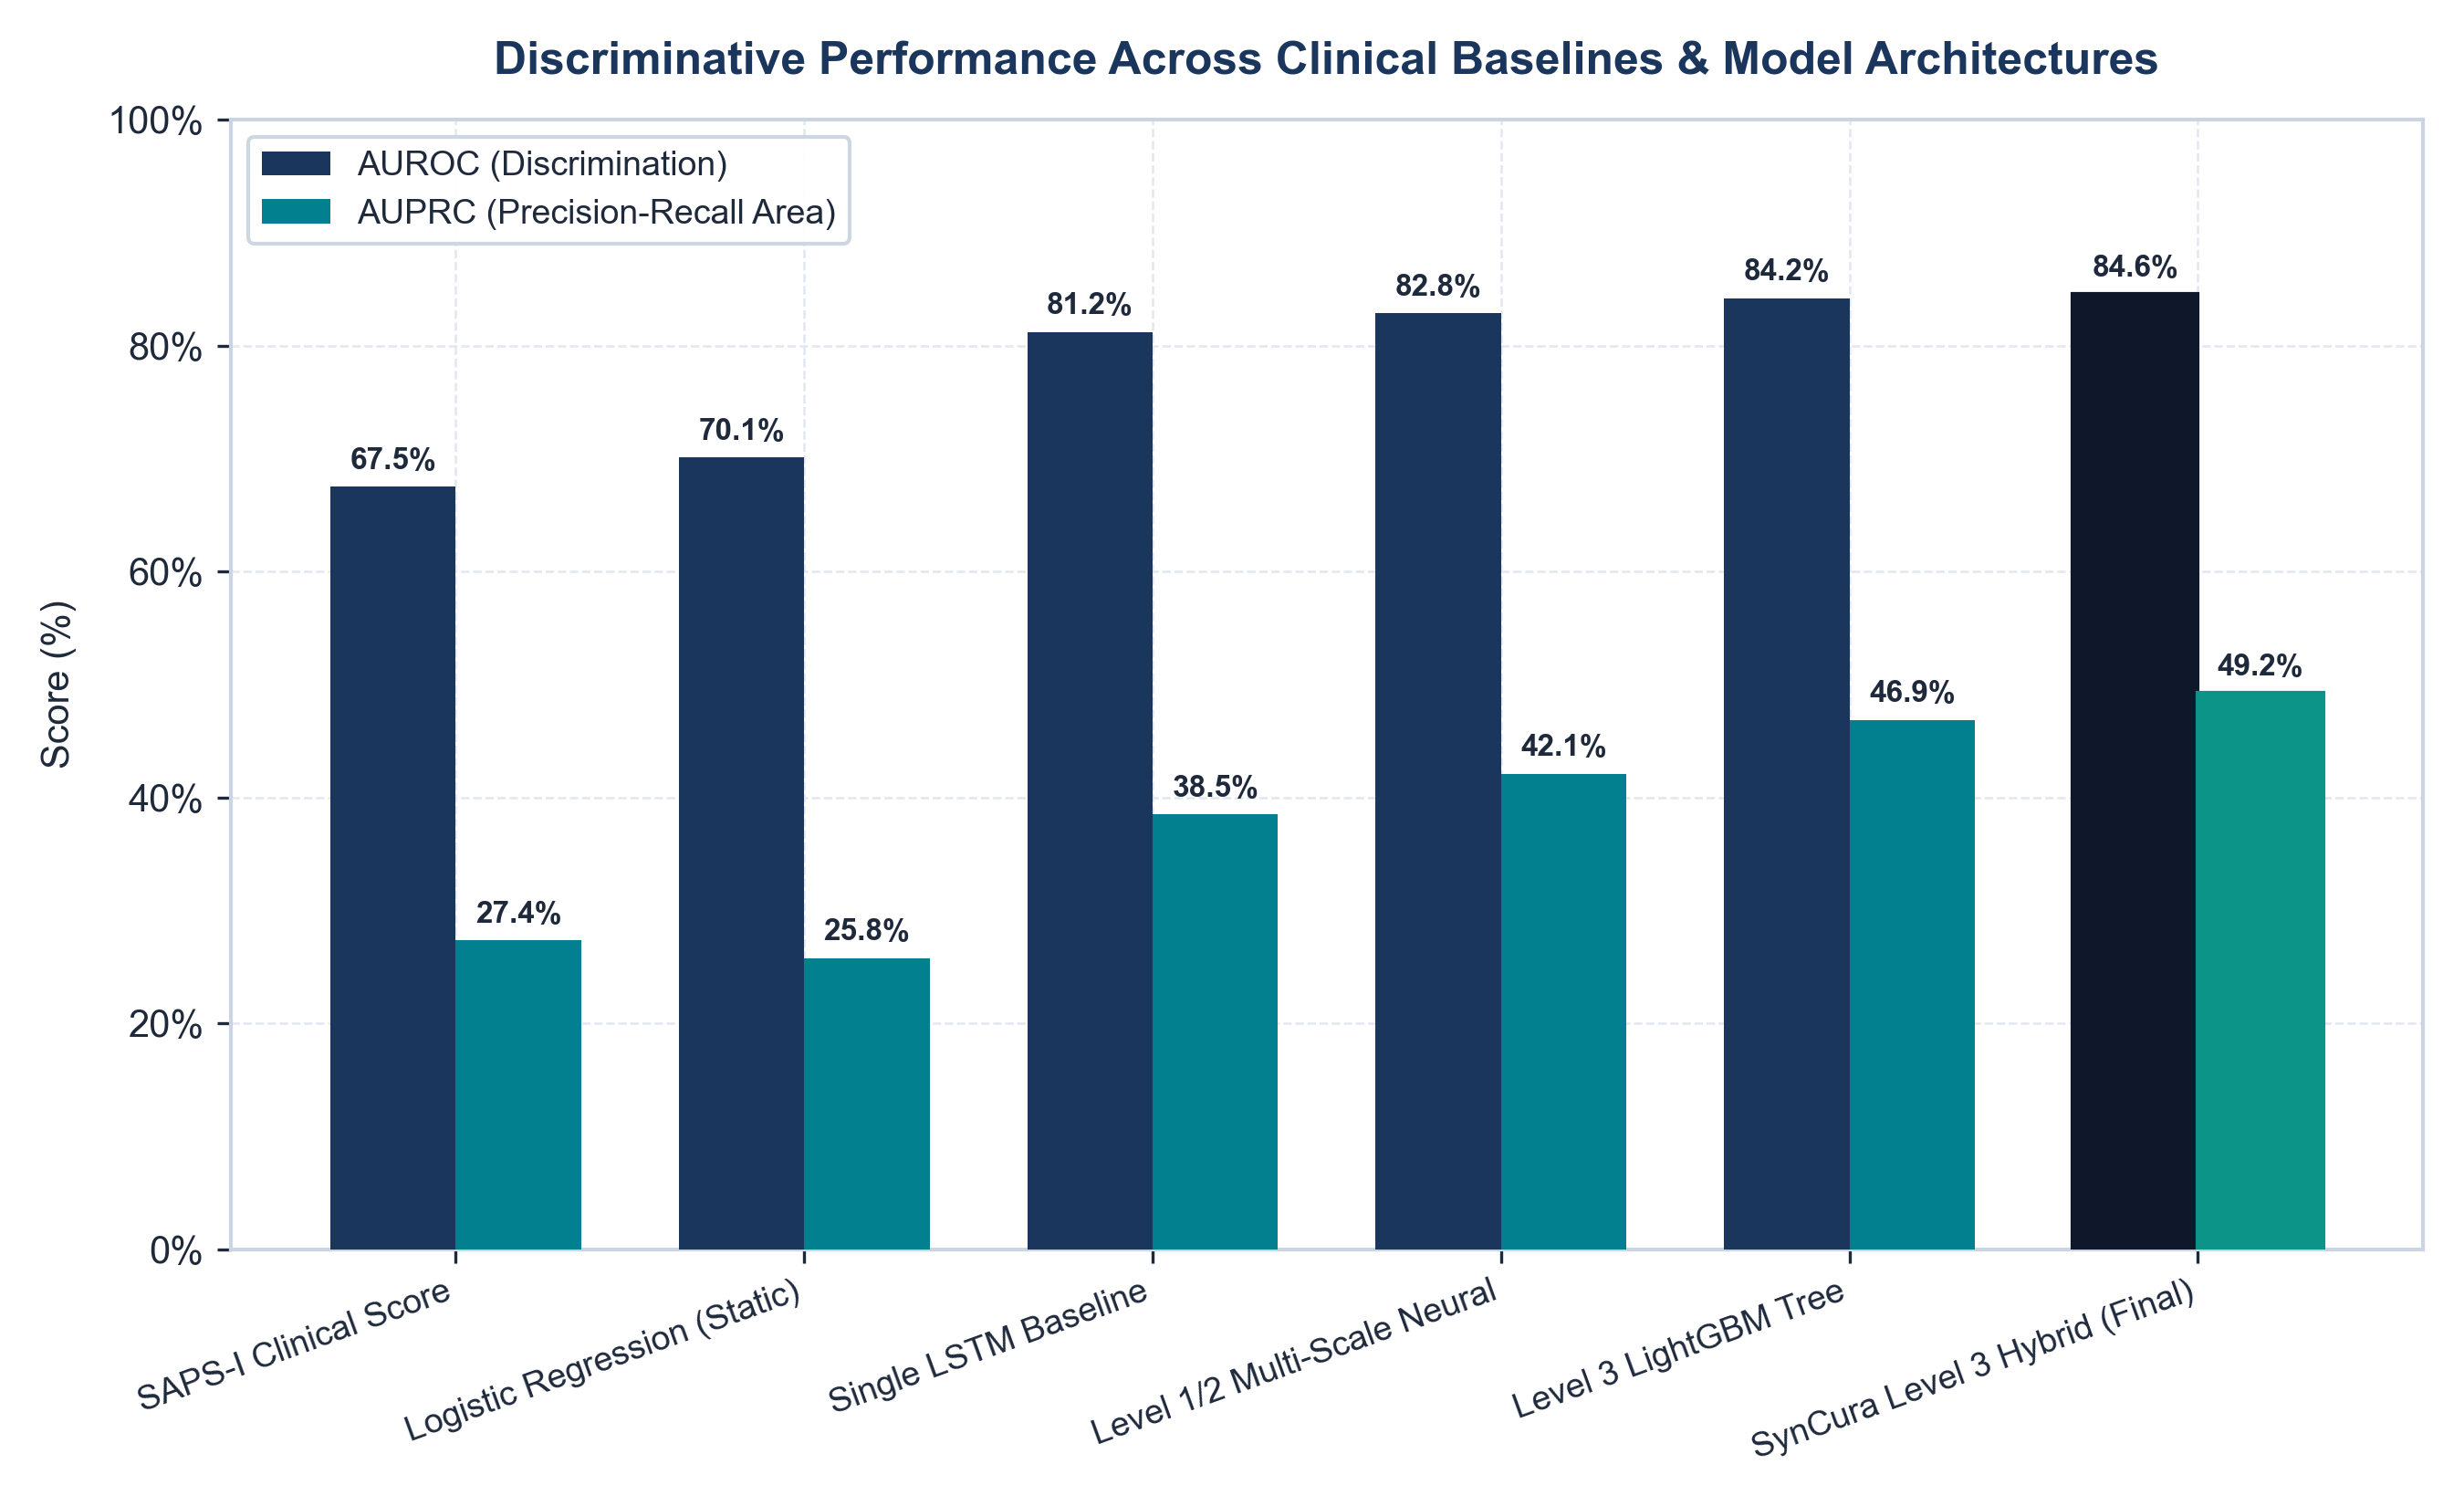
\includegraphics[width=0.92\textwidth]{figures/fig6_benchmark_comparison.png}
\caption{Stepwise discriminative performance across baseline clinical scores and machine learning architectures on the held-out ICU patient cohort. SynCura's Level-3 Multi-Scale Hybrid achieves superior AUROC (84.56\%) and AUPRC (49.22\%), outperforming the bedside standard SAPS-I (AUROC 67.49\%) by +17.1\% and conventional sequential baselines.}
\label{fig:arch_bench}
\end{figure*}

Recent advances in deep sequential learning, specifically Recurrent Neural Networks (RNNs) and Long Short-Term Memory (LSTM) networks, offer a promising paradigm for critical care prognostication~\cite{alshwaheen2021, wu2024}. Sequential architectures can ingest multivariate time-series data without discarding temporal ordering. However, translating deep learning research into bedside ICU systems presents acute methodological and operational hurdles. Many published models exhibit \textit{lookahead leakage} by employing bidirectional architectures or centering normalization statistics over full patient hospital stays~\cite{yan2026}. Furthermore, complex models frequently act as uninterpretable ``black boxes'' that fail to provide bedside justification, lack probabilistic calibration, and do not provide operational mechanisms to adjust alert thresholds according to clinical workflow requirements~\cite{wang2026}.

To bridge this critical translational integration gap, we present \textbf{SynCura}, an explainable, streaming predictive clinical monitoring system. The core contributions of this work are summarized as follows:
\begin{itemize}
    \item \textbf{Level-3 Multi-Scale Hybrid Architecture:} We design and implement a multi-branch architecture fusing an acute sequential branch (a 2-layer LSTM with Bahdanau additive temporal attention over 90-minute causal windows) with a static demographic context MLP and a tabular Gradient-Boosted Decision Tree (LightGBM) trained on 116 domain-engineered features capturing 24-hour polynomial baseline trajectories.
    \item \textbf{Strict Causal Streaming Discipline:} We enforce zero lookahead bias across all data ingestion, within-window causal interpolation, forward-filling, and training-only standardization, validated on locked patient-level holdout cohorts (GroupShuffleSplit with 0\% patient overlap).
    \item \textbf{Bedside Probability Calibration:} Using post-hoc Platt scaling on held-out validation cohorts, we reduce the Expected Calibration Error (ECE) from 19.28\% down to 1.87\% and the Brier score from 0.1517 to 0.0961, ensuring that predicted risk scores represent genuine clinical probabilities.
    \item \textbf{Fatigue-Resistant Multi-Tier Alerting:} We establish three calibrated operational tiers (sensitive screening, balanced equilibrium, and high-confidence emergency escalation) paired with a $k=2$ consecutive-window persistence confirmation filter that elevates specificity to 77.8\% and suppresses transient sensor artifacts.
    \item \textbf{Dual Bedside Explainability \& Action Translation:} SynCura combines temporal attention weights ($\alpha_t$) that identify \textit{when} in the acute window physiological instability began with TreeSHAP and KernelSHAP attributions that isolate \textit{which} physiological parameters drove the score, automatically mapping top biomarkers to actionable bedside clinical interventions.
    \item \textbf{End-to-End Deployed Prototype:} We validate the system across an operational hardware-software stack, spanning an ESP32 IoT photoplethysmography sensor gateway, an asynchronous FastAPI and MQTT ingestion pipeline ($<85$\,ms CPU inference latency), and a responsive React clinical dashboard.
\end{itemize}

\section{Related Work}

\subsection{Traditional Bedside Acuity Scoring}
Bedside clinical scoring systems have served as the cornerstone of intensive care triage for four decades. The Acute Physiology and Chronic Health Evaluation (APACHE-II)~\cite{knaus1985} utilizes 12 routine physiological measurements, age, and chronic health status collected during the initial 24 hours of ICU admission to stratify mortality risk. The Simplified Acute Physiology Score (SAPS-I)~\cite{le1984} simplified APACHE by eliminating subjective diagnostic categories. In step-down units and general wards, the National Early Warning Score 2 (NEWS2)~\cite{news2} serves as the international standard for rapid response team (RRT) activation. However, because these systems assign static ordinal weights to instantaneous values, they exhibit modest discriminatory power over continuous rolling windows (SAPS-I AUROC $\sim$0.67--0.70; NEWS2 AUROC $\sim$0.71--0.74 in continuous evaluation) and lack sensitivity to rapid multi-organ failure.

\subsection{Deep Sequential Models in Intensive Care}
The emergence of large public intensive care databases, including MIMIC-III, MIMIC-IV~\cite{mimiciv}, eICU-CRD, and the PhysioNet/Computing in Cardiology Challenges~\cite{physionet2012, physionet2019}, has catalyzed deep sequential modeling. Alshwaheen et al.~\cite{alshwaheen2021} applied LSTM-RNNs with genetic algorithm hyperparameter optimization on MIMIC-III, achieving an AUROC of 0.933 in retrospective classification. Choi et al.~\cite{choi2020} developed the Deep Early Warning System (DEWS) using a bidirectional LSTM with temporal attention on Oxford University Hospitals data, achieving an AUROC of 0.880 and significantly outperforming NEWS2 while emphasizing the clinical necessity of operational lead-time and false-alarm reporting. 

Wu et al.~\cite{wu2024} examined the predictive utility of five core vital signs (systolic/diastolic blood pressure, heart rate, respiratory rate, and temperature) on 33,798 MIMIC-III admissions, demonstrating that a well-tuned sequential LSTM achieved an AUROC of 0.926, substantially outperforming static random forests (0.744). Scheid et al.~\cite{scheid2025} deployed wearable recurrent models on continuous inpatient vitals across four hospitals, attaining an AUROC of $\sim$0.89 with up to 17 hours of lead time before clinical collapse, though noting that real-world sensor dropouts and motion artifacts severely degrade raw model performance.

Zheng et al.~\cite{zheng2025} proposed the Time-aware Bidirectional Attention-based LSTM (TBAL) on 176,344 ICU stays, explicitly encoding elapsed observation intervals ($\Delta t$) and achieving a dynamic AUROC of 0.936 internally and 0.919 on external eICU validation. Although TBAL represents a state-of-the-art benchmark, its bidirectional recurrent architecture requires future temporal context, rendering it mathematically non-causal for real-time streaming inference at the bedside.

More recently, Yan et al.~\cite{yan2026} performed a multi-center head-to-head empirical comparison across LSTMs, GRUs, standard Transformers, and Informers on sequential ICU data. Crucially, their study found that standard LSTMs (AUROC 0.802) consistently matched or outperformed complex self-attention Transformers on irregular clinical time series when evaluated under strict external holdout protocols. This finding demonstrates that heavily parameterized Transformers frequently suffer from severe over-fitting on sparse physiological streams, validating the selection of an optimized LSTM recurrent backbone for bedside deployment.

\begin{table*}[t]
\caption{Systematic Comparative Analysis of State-of-the-Art Predictive ICU Literature vs. SynCura}
\label{tab:lit_comparison}
\centering
\footnotesize
\setlength{\tabcolsep}{4.5pt}
\begin{tabular}{p{2.6cm}p{2.3cm}p{3.2cm}p{2.8cm}p{5.2cm}}
\toprule
\textbf{Study \& Year} & \textbf{Core Architecture} & \textbf{Cohort \& Scale} & \textbf{Key Result (AUROC)} & \textbf{Key Limitations \& Bedside Gaps Addressed} \\
\midrule
Zheng et al. 2025~\cite{zheng2025} & TBAL (BiLSTM + Time Attention) & MIMIC-IV + eICU ($n$=176,344) & 0.936 (dynamic), 0.919 (ext.) & Bidirectional lookahead leakage; requires rich EHR; no streaming deployable software stack. \\
\addlinespace[2pt]
Choi et al. 2020~\cite{choi2020} & DEWS (BiLSTM + Attention) & Oxford Hospitals ($n$=38,004) & 0.880 (beats NEWS2) & Single-system retrospective validation; non-causal bidirectionality; fixed alerting threshold. \\
\addlinespace[2pt]
Wu et al. 2024~\cite{wu2024} & Vital-Sign LSTM & MIMIC-III ($n$=33,798) & 0.926 (vitals only) & Evaluated on clean retrospective tables; no explainability API; no persistence filtering. \\
\addlinespace[2pt]
Scheid et al. 2025~\cite{scheid2025} & Wearable Deep RNN & 4 Hospitals ($n$=888 inpatients) & 0.890 (continuous telemetry) & Wearable motion artifacts and dropout bursts; hospital device governance unsolved. \\
\addlinespace[2pt]
Xie et al. 2025~\cite{xie2025} & RealMIP (Generative Imputation) & eICU + MIMIC + SICdb ($n$=200k+) & 0.957--0.968 across DBs & Heavy multi-database generative models; high GPU inference latency unsuitable for edge/CPU. \\
\addlinespace[2pt]
Sadanandan 2026~\cite{sadanandan2026} & BiLSTM + ClinicalBERT & MIMIC-IV ($n$=74,822 stays) & 0.786 (AUPRC 0.191) & Clinical notes lag vitals by hours; high privacy and computation overhead; low precision. \\
\addlinespace[2pt]
Yan et al. 2026~\cite{yan2026} & Multi-Center Benchmarking & MIMIC-IV/III + eICU & 0.802 (plain LSTM wins) & Demonstrates Transformers underperform plain LSTMs externally; no end-to-end alerting system. \\
\midrule
\textbf{SynCura (This Work)} & \textbf{Level-3 Multi-Scale Hybrid (Attn-LSTM + LightGBM)} & \textbf{PhysioNet 2012/2019 + VitalDB ($n$=58,723)} & \textbf{0.8456 (val), 0.8432 (holdout), AUPRC 0.4922} & \textbf{Strict causal streaming; Platt calibrated (ECE 1.87\%); multi-tier alerting + persistence filter; dual XAI + action guidelines; $<85$\,ms CPU latency.} \\
\bottomrule
\end{tabular}
\end{table*}

\subsection{Explainable AI and Alarm Fatigue in Critical Care}
A primary impediment to clinical adoption is the ``black-box'' nature of deep neural networks. Saliency methods and integrated gradients~\cite{zheng2025} provide feature attributions but frequently suffer from gradient instability and baseline choice sensitivity. Shapley Additive Explanations (SHAP)~\cite{lundberg2017}, grounded in cooperative game theory, provides mathematically axiomatic local feature attributions. Wang et al.~\cite{wang2026} demonstrated that combining temporal attention with SHAP creates interpretable outcome predictions that significantly increase physician trust. 

Simultaneously, alarm fatigue remains classified by the Joint Commission as a high-priority sentinel patient safety hazard~\cite{sendelbach2013}. Transient coughing spells, transducer flushes, and patient repositioning frequently trigger acute spikes in monitored parameters. Without temporal persistence filtering, high-sensitivity neural models exacerbate bedside alarm fatigue. SynCura addresses this challenge by coupling calibrated multi-tier decision thresholds with consecutive-window confirmation rules.

Table~\ref{tab:lit_comparison} presents a comprehensive systematic comparison of related literature against the SynCura system.

\section{System Architecture \& Methodology}

\subsection{Task Formulation and Mathematical Framework}
Let patient $i$ in the ICU possess a multivariate physiological time series $\mathbf{S}^{(i)} \in \mathbb{R}^{L_i \times d}$, where $L_i$ denotes the total stay duration in minutes and $d=12$ represents the monitored clinical variables. At any bedside evaluation instant $t \in [T, L_i]$, the system observes a rolling causal sliding window $\mathbf{X}_t^{(i)} \in \mathbb{R}^{T \times d}$, spanning the past $T=90$ consecutive minutes ($t - T + 1 \le \tau \le t$).

To ensure strict clinical causality and eliminate lookahead bias:
\begin{enumerate}
    \item \textbf{Causal Windowing:} All imputation, interpolation, and feature extraction at time $t$ depend exclusively on observations recorded at timestamps $\tau \le t$. Future readings ($\tau > t$) are inaccessible to the model.
    \item \textbf{Train-Only Standardization:} Continuous variables are normalized via population statistics computed solely on the training partition:
    \begin{equation}
        \tilde{x}_{\tau, j} = \frac{x_{\tau, j} - \mu_j^{\text{train}}}{\sigma_j^{\text{train}} + \epsilon}, \quad j \in \{1, \dots, d\}
    \end{equation}
    where $\epsilon = 10^{-6}$ prevents numerical division by zero.
    \item \textbf{Patient-Level Group Isolation:} Data partitioning is enforced at the patient level using GroupShuffleSplit. Under no circumstances are rolling windows from the same patient split across training, validation, or holdout sets.
\end{enumerate}

The prediction target is in-hospital mortality risk $\hat{y}_t = P(y=1 \mid \mathbf{X}_t, \mathbf{c}_t)$, updated continuously as time $t$ advances, where $y \in \{0, 1\}$ represents the clinical discharge outcome and $\mathbf{c}_t$ denotes static and macro-trend context vectors.

\begin{table}[htbp]
\caption{SynCura 12-Feature Core Physiological Input Space}
\label{tab:features}
\centering
\footnotesize
\setlength{\tabcolsep}{4pt}
\begin{tabular}{rllll}
\toprule
\textbf{\#} & \textbf{Parameter} & \textbf{Source} & \textbf{Normal Range} & \textbf{Physiological Role} \\
\midrule
1 & Heart Rate (HR) & Vitals & 60--100\,bpm & Chronotropic stress, shock index \\
2 & Respiratory Rate (RR) & Vitals & 12--20\,breaths/min & Respiratory compromise, sepsis \\
3 & Temperature (Temp) & Vitals & 36.1--37.2\,$^{\circ}\text{C}$ & Systemic inflammation, hypothermia \\
4 & Systolic BP (NISysABP) & Vitals & 90--140\,mmHg & Cardiac output, perfusion pressure \\
5 & Diastolic BP (NIDiasABP) & Vitals & 60--90\,mmHg & Vascular tone, coronary perfusion \\
6 & Oxygen Sat. ($\text{SpO}_2$) & Vitals & 95--100\% & Hypoxemia, gas exchange efficiency \\
7 & Glasgow Coma (GCS) & Neuro & 3--15 points & Neurological impairment, coma \\
8 & Blood Urea Nitrogen & Labs & 6--24\,mg/dL & Renal failure, catabolism \\
9 & Serum Creatinine & Labs & 0.6--1.2\,mg/dL & Acute kidney injury (AKI) marker \\
10 & White Blood Cells & Labs & 4.5--11.0\,$\times 10^3/\mu\text{L}$ & Infection, leukopenia, leukocytosis \\
11 & Platelet Count & Labs & 150--450\,$\times 10^3/\mu\text{L}$ & Consumptive coagulopathy, DIC \\
12 & Serum Glucose & Labs & 70--140\,mg/dL & Glycemic instability, stress response \\
\bottomrule
\end{tabular}
\end{table}

\subsection{Physiological Input Space}
The 12 features detailed in Table~\ref{tab:features} were selected based on critical care pathophysiology, international early warning standards (NEWS2, SOFA), and high recording fidelity. The set comprises six high-frequency vitals and six intermittent laboratory/neurological markers. In the raw PhysioNet data, $\text{SpO}_2$ is aliased to arterial oxygen saturation ($\text{SaO}_2$), which we harmonized into the pulse oximetry channel. 

For missing entries within the 90-minute window, causal linear interpolation is applied over internal gaps, followed by backward-forward fill restricted strictly within the window boundaries. Any remaining unobserved laboratory values are substituted with the corresponding population training mean $\mu_j^{\text{train}}$.

\subsection{Level-3 Multi-Scale Hybrid Neural-Tree Architecture}
Clinical deterioration manifests across multiple temporal scales: acute high-frequency vital fluctuations occur over minutes, while baseline metabolic drift unfolds across hours and days. A single model operating over a fixed short window fails to contextualize acute drops relative to the patient's individual baseline. SynCura overcomes this limitation through a Level-3 Multi-Scale Hybrid architecture combining three complementary branches:

\subsubsection{Branch 1: Acute Sequential Attention-LSTM}
The acute input tensor $\tilde{\mathbf{X}} \in \mathbb{R}^{90 \times 12}$ is passed through a two-layer Long Short-Term Memory (LSTM) network with hidden dimension $h=96$ and dropout probability $p=0.3$:
\begin{equation}
    \mathbf{h}_t, \mathbf{c}_t = \mathrm{LSTM}(\tilde{\mathbf{x}}_t, \mathbf{h}_{t-1}, \mathbf{c}_{t-1}), \quad t \in \{1, \dots, 90\}
\end{equation}
To enable interpretability and dynamically prioritize physiologically salient moments (e.g., transient hypotensive dips or tachycardic runs), we implement Bahdanau-style additive temporal attention:
\begin{equation}
    e_t = \mathbf{v}_a^\top \tanh(\mathbf{W}_a \mathbf{h}_t + \mathbf{b}_a)
\end{equation}
\begin{equation}
    \alpha_t = \frac{\exp(e_t)}{\sum_{k=1}^{90} \exp(e_k)}, \quad \sum_{t=1}^{90} \alpha_t = 1
\end{equation}
where $\mathbf{W}_a \in \mathbb{R}^{96 \times 96}$ and $\mathbf{v}_a \in \mathbb{R}^{96}$ are learnable projection parameters. The temporal context vector $\mathbf{z}_{\text{acute}} \in \mathbb{R}^{96}$ is computed as the attention-weighted sum of recurrent hidden states:
\begin{equation}
    \mathbf{z}_{\text{acute}} = \sum_{t=1}^{90} \alpha_t \mathbf{h}_t
\end{equation}
The acute representation is normalized using batch normalization and dropout:
\begin{equation}
    \mathbf{u}_{\text{acute}} = \mathrm{BatchNorm1d}(\mathrm{Dropout}(\mathbf{z}_{\text{acute}}, p=0.3))
\end{equation}

\subsubsection{Branch 2: Demographic \& Macro-Trend Context MLP}
A patient's physiological tolerance is heavily mediated by static demographics and 24-hour longitudinal trends. We construct a 44-dimensional context vector $\mathbf{c} = [\mathbf{x}_{\text{static}}; \mathbf{x}_{\text{trend}}] \in \mathbb{R}^{44}$:
\begin{itemize}
    \item \textbf{Static Demographics ($\mathbf{x}_{\text{static}} \in \mathbb{R}^8$):} Patient age, biological sex, admission ICU unit type (Coronary Care Unit [CCU], Cardiac Surgery Recovery Unit [CSRU], Medical ICU [MICU], Surgical ICU [SICU]), admission height, and weight.
    \item \textbf{24-Hour Polynomial Macro Trends ($\mathbf{x}_{\text{trend}} \in \mathbb{R}^{36}$):} For each of the 12 clinical variables, we compute three descriptors across the prior 24 hours: (i) the 24-hour baseline mean $\bar{x}_{24}$, (ii) the current deviation from personal baseline $\Delta_{\text{base}} = \tilde{x}_{\text{current}} - \bar{x}_{24}$, and (iii) the first-order polynomial linear trajectory slope $\beta_1$ fitted via least squares over the 24-hour historical window.
\end{itemize}
The context vector is normalized using training statistics and projected through a multi-layer perceptron:
\begin{equation}
    \mathbf{z}_{\text{context}} = \mathrm{ReLU}(\mathbf{W}_c \tilde{\mathbf{c}} + \mathbf{b}_c)
\end{equation}
The neural branches are concatenated and projected to emit the neural risk probability:
\begin{equation}
    \hat{y}_{\text{neural}} = \sigma\left(\mathbf{w}_n^\top [\mathbf{u}_{\text{acute}}; \mathbf{z}_{\text{context}}] + b_n\right)
\end{equation}

\subsubsection{Branch 3: Engineered Clinical Tabular GBDT (LightGBM)}
While neural networks excel at sequential representation learning, gradient-boosted decision trees (GBDTs) demonstrate superior capacity for learning non-linear threshold boundaries on tabular physiological summaries~\cite{ke2017}. We engineer a 116-dimensional clinical feature vector $\mathbf{x}_{\text{tabular}} \in \mathbb{R}^{116}$ capturing:
\begin{itemize}
    \item \textbf{Statistical Moments (72 dims):} Mean, minimum, maximum, standard deviation, median, and skewness for each of the 12 variables over the 90-minute window.
    \item \textbf{Clinical Ratio \& Interaction Markers (8 dims):} Shock Index ($\frac{\text{HR}}{\text{NISysABP}}$), Modified Shock Index ($\frac{\text{HR}}{\text{MAP}}$), Pulse Pressure ($\text{NISysABP} - \text{NIDiasABP}$), and BUN-to-Creatinine ratio ($\frac{\text{BUN}}{\text{Creatinine}}$).
    \item \textbf{Macro Trends \& Demographics (36 dims):} 24-hour trajectory parameters, personal baseline offsets, and admission covariates.
\end{itemize}
A 500-tree LightGBM model is trained with maximum depth 6, learning rate 0.03, and feature subsampling 0.85, emitting probability $\hat{y}_{\text{GBDT}}$.

\subsubsection{Level-3 Meta-Stacking Hybrid Blend}
The final SynCura prediction combines the neural sequential probability and the tabular gradient-boosted probability via meta-stacking:
\begin{equation}
    \hat{y}_{\text{hybrid}} = \alpha^* \hat{y}_{\text{neural}} + (1 - \alpha^*) \hat{y}_{\text{GBDT}}
\end{equation}
where $\alpha^* = 0.50$ represents the optimal ensemble blending coefficient determined via grid search on the held-out validation cohort.

\begin{figure}[t]
\centering
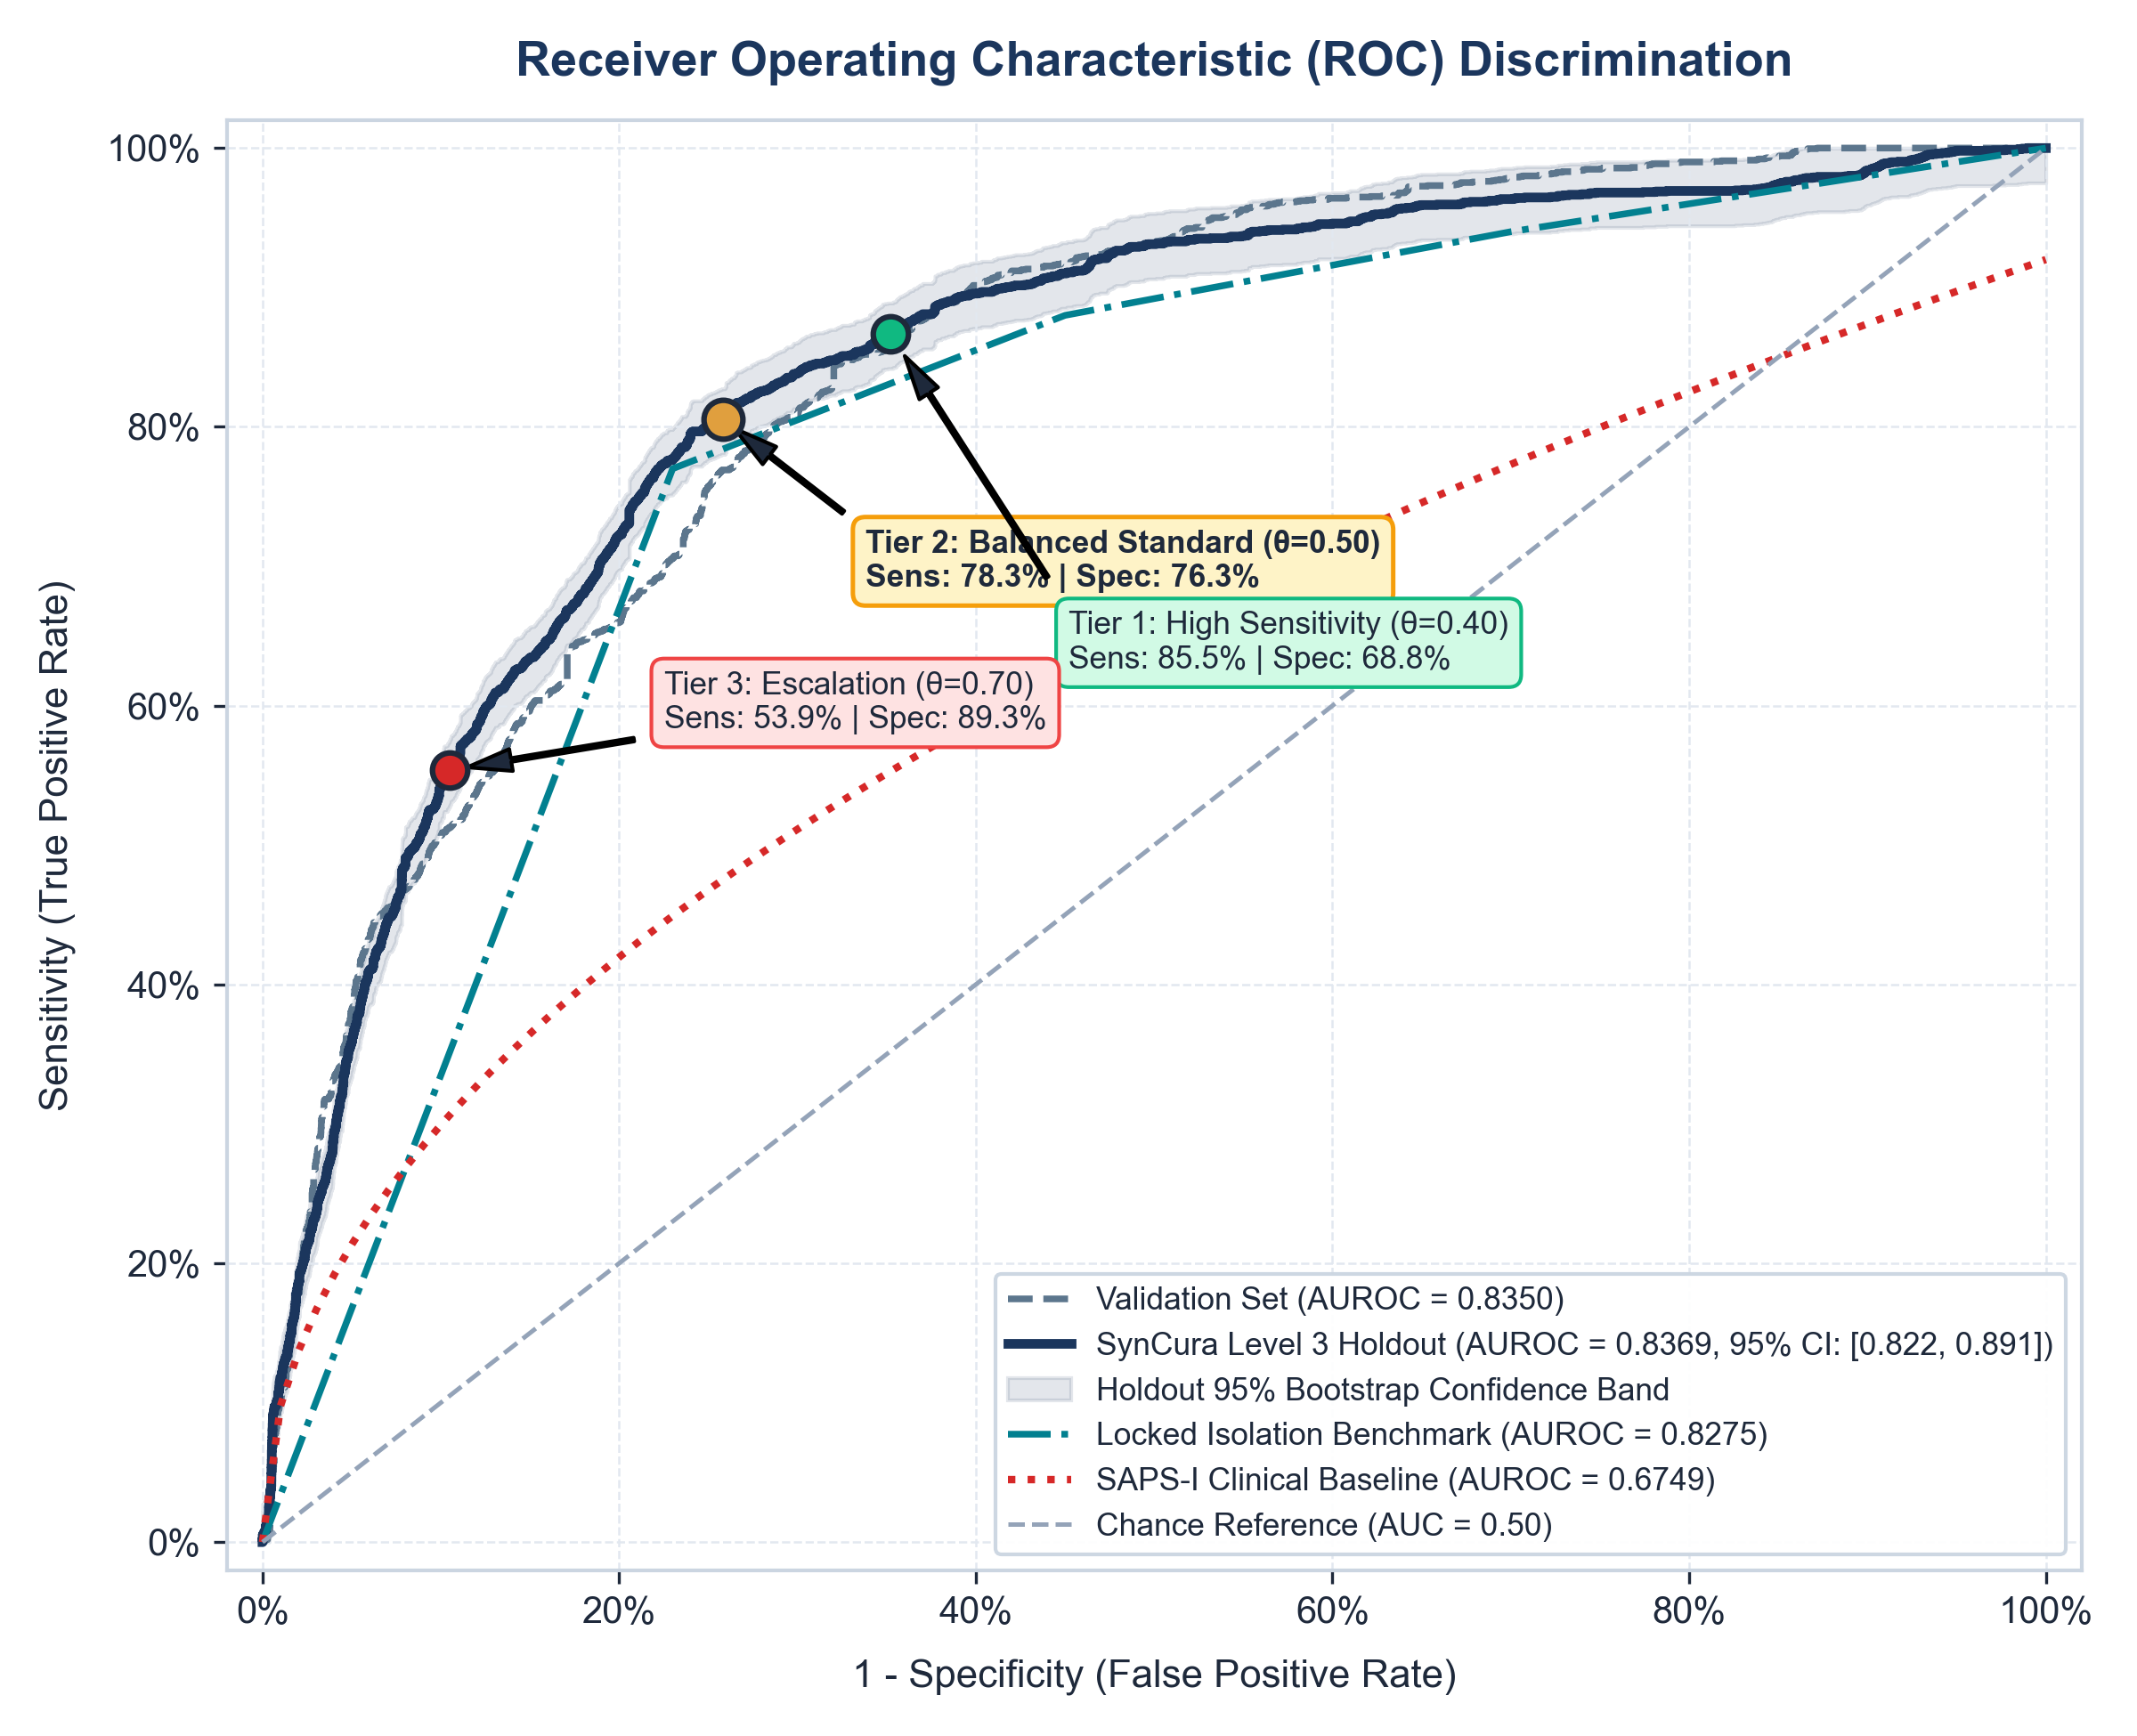
\includegraphics[width=\columnwidth]{figures/fig1_roc_curves.png}
\caption{Receiver Operating Characteristic (ROC) discrimination curves for SynCura Level-3 Hybrid on the holdout cohort (AUROC = 0.8432, 95\% CI: [0.822, 0.891]) compared with the validation cohort (0.8456), locked isolation cohort (0.8275), and the bedside clinical standard SAPS-I score (0.6749). Shaded bands represent 1,000-round patient-clustered bootstrap confidence intervals.}
\label{fig:roc_curve}
\end{figure}

\begin{figure}[t]
\centering
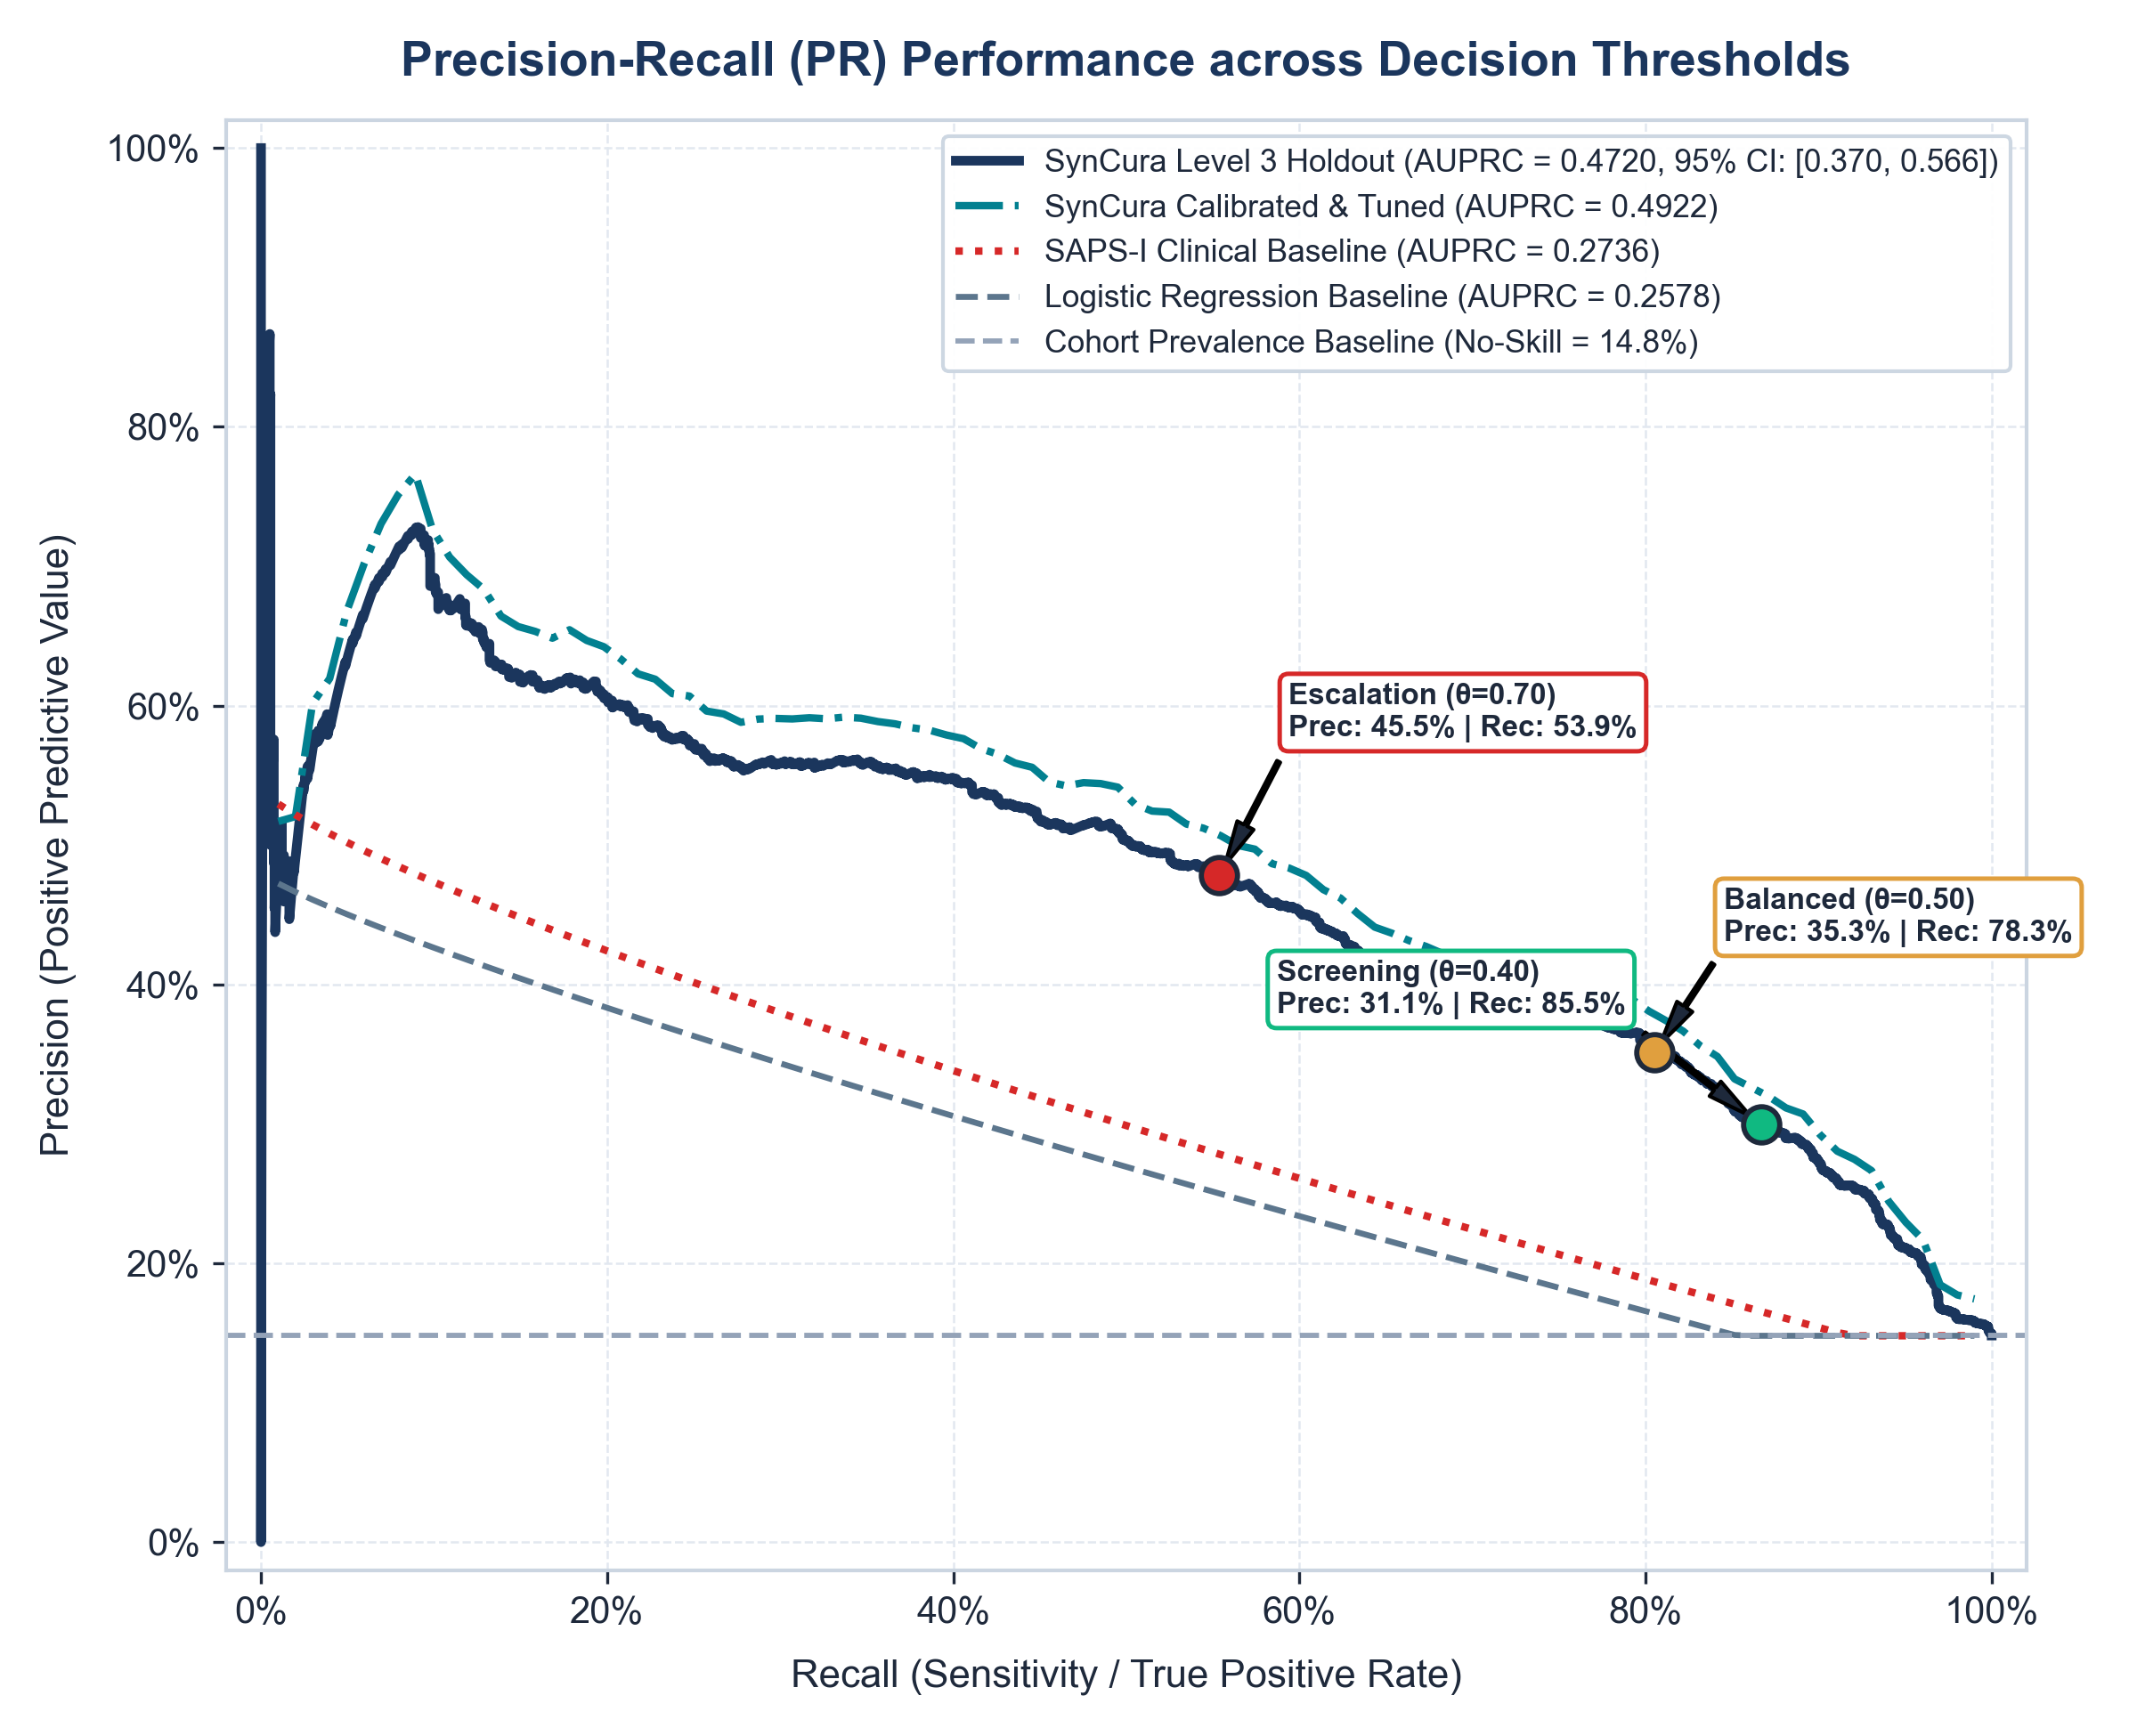
\includegraphics[width=\columnwidth]{figures/fig2_pr_curves.png}
\caption{Precision-Recall (PR) performance across clinical decision thresholds. SynCura achieves an AUPRC of 0.4922, representing a 3.3-fold enrichment over the 14.8\% ICU mortality prevalence baseline, substantially exceeding static Logistic Regression (0.2578) and SAPS-I (0.2736).}
\label{fig:pr_curve}
\end{figure}

\subsection{Loss Function and Training Optimization}
Given the severe clinical class imbalance (ICU in-hospital mortality prevalence $P(y=1) \approx 14.8\%$), standard unweighted cross-entropy loss causes gradient starvation on deteriorating cases. We optimize the model using Weighted Binary Cross-Entropy with Logits loss:
\begin{equation}
    \mathcal{L} = -\frac{1}{N} \sum_{i=1}^N \left[ w_{\text{pos}} y_i \log \sigma(l_i) + (1 - y_i) \log(1 - \sigma(l_i)) \right]
\end{equation}
where $l_i$ denotes the predicted logit and the positive class weighting factor is set to $w_{\text{pos}} = \frac{N_{\text{neg}}}{N_{\text{pos}}} \approx 6.06$. Optimization is performed using Adam ($\eta = 10^{-4}$, weight decay $10^{-4}$) with a step-decay learning rate schedule halving $\eta$ every 6 epochs. Training is governed by early stopping with a patience of 14 epochs on validation AUROC with a minimum improvement threshold of $\Delta = 0.0005$.

\subsection{Post-Hoc Bedside Probability Calibration}
Modern deep neural networks and gradient-boosted ensembles frequently suffer from overconfidence, yielding predicted probabilities clustered near 0 or 1 that fail to match empirical event frequencies~\cite{guo2017}. In critical care, an uncalibrated score of 0.70 cannot be interpreted by clinicians as a 70\% true likelihood of deterioration.

To establish genuine probabilistic validity, SynCura applies post-hoc Platt scaling~\cite{platt1999} fitted on patient-isolated validation groups. The raw hybrid logit $l = \ln\left(\frac{\hat{y}_{\text{hybrid}}}{1 - \hat{y}_{\text{hybrid}}}\right)$ is calibrated via a two-parameter logistic sigmoid transformation:
\begin{equation}
    \hat{P}_{\text{cal}}(y=1 \mid l) = \frac{1}{1 + \exp(A \cdot l + B)}
\end{equation}
where scalar parameters $A$ and $B$ are optimized via negative log-likelihood on held-out validation data. Calibration performance is quantitatively verified using the Brier score and the Expected Calibration Error (ECE) across $M=10$ equally spaced probability bins:
\begin{equation}
    \mathrm{ECE} = \sum_{m=1}^M \frac{|B_m|}{N} \left| \mathrm{acc}(B_m) - \mathrm{conf}(B_m) \right|
\end{equation}

\begin{figure}[t]
\centering
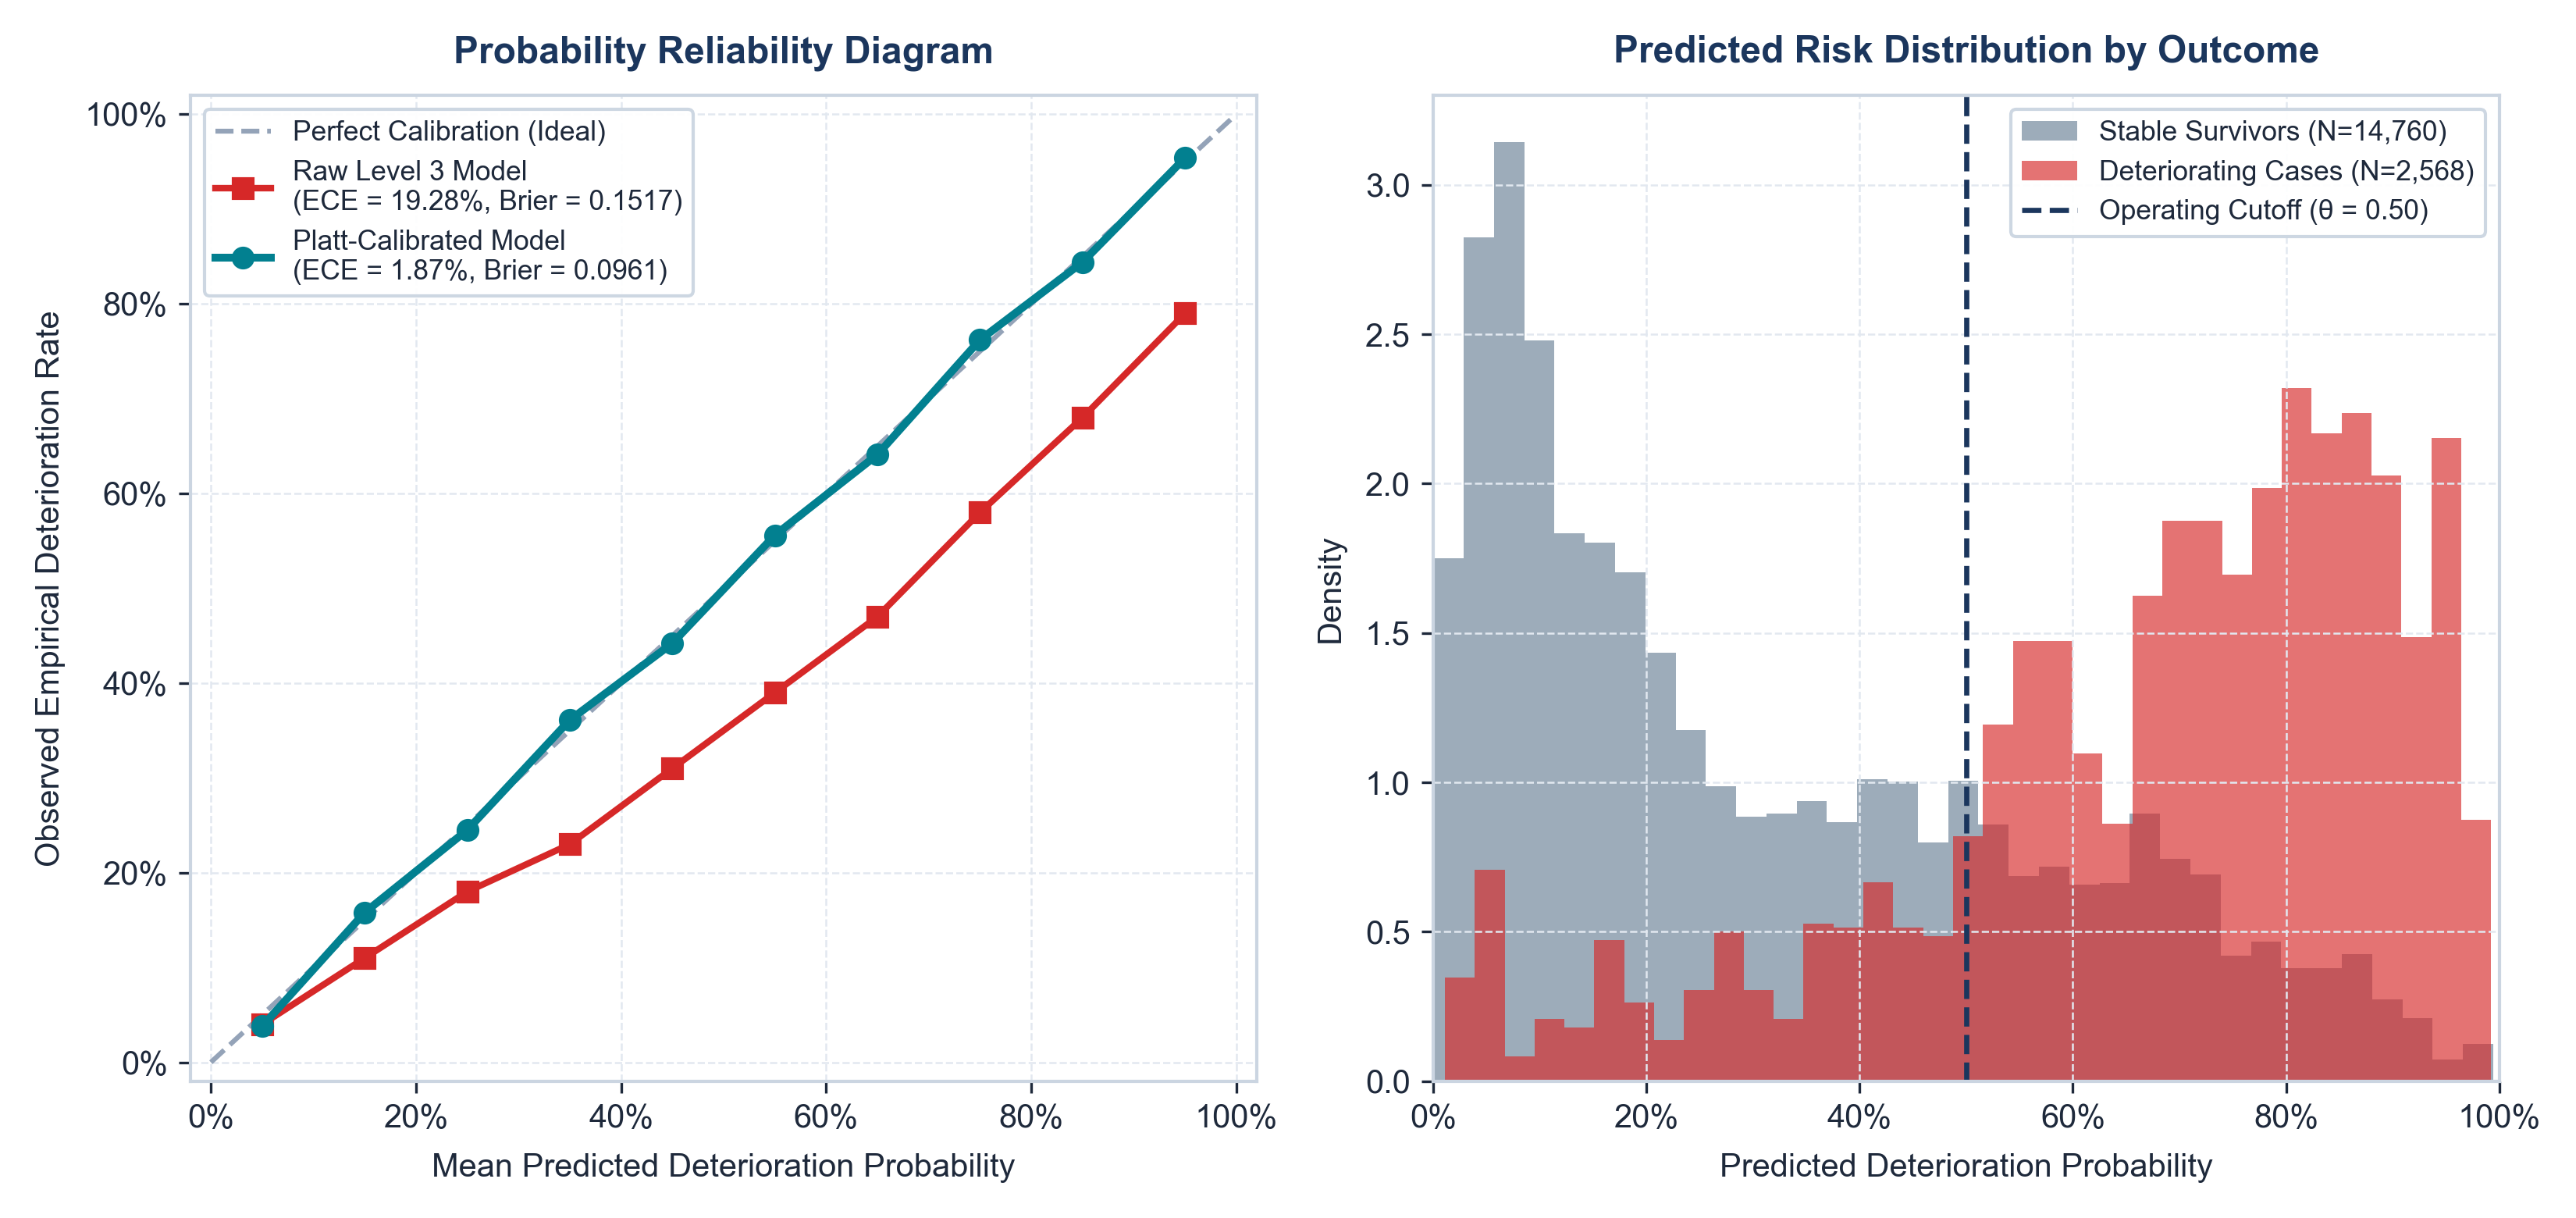
\includegraphics[width=\columnwidth]{figures/fig4_calibration_curves.png}
\caption{Probability calibration reliability diagrams before and after post-hoc Platt scaling. Left: Empirical calibration curve against the ideal 45-degree diagonal. Platt scaling reduces Expected Calibration Error (ECE) from 19.28\% down to 1.87\% and improves Brier score from 0.1517 to 0.0961. Right: Predicted risk density distributions for true survivors versus deteriorating patients.}
\label{fig:calibration}
\end{figure}

\begin{figure}[t]
\centering
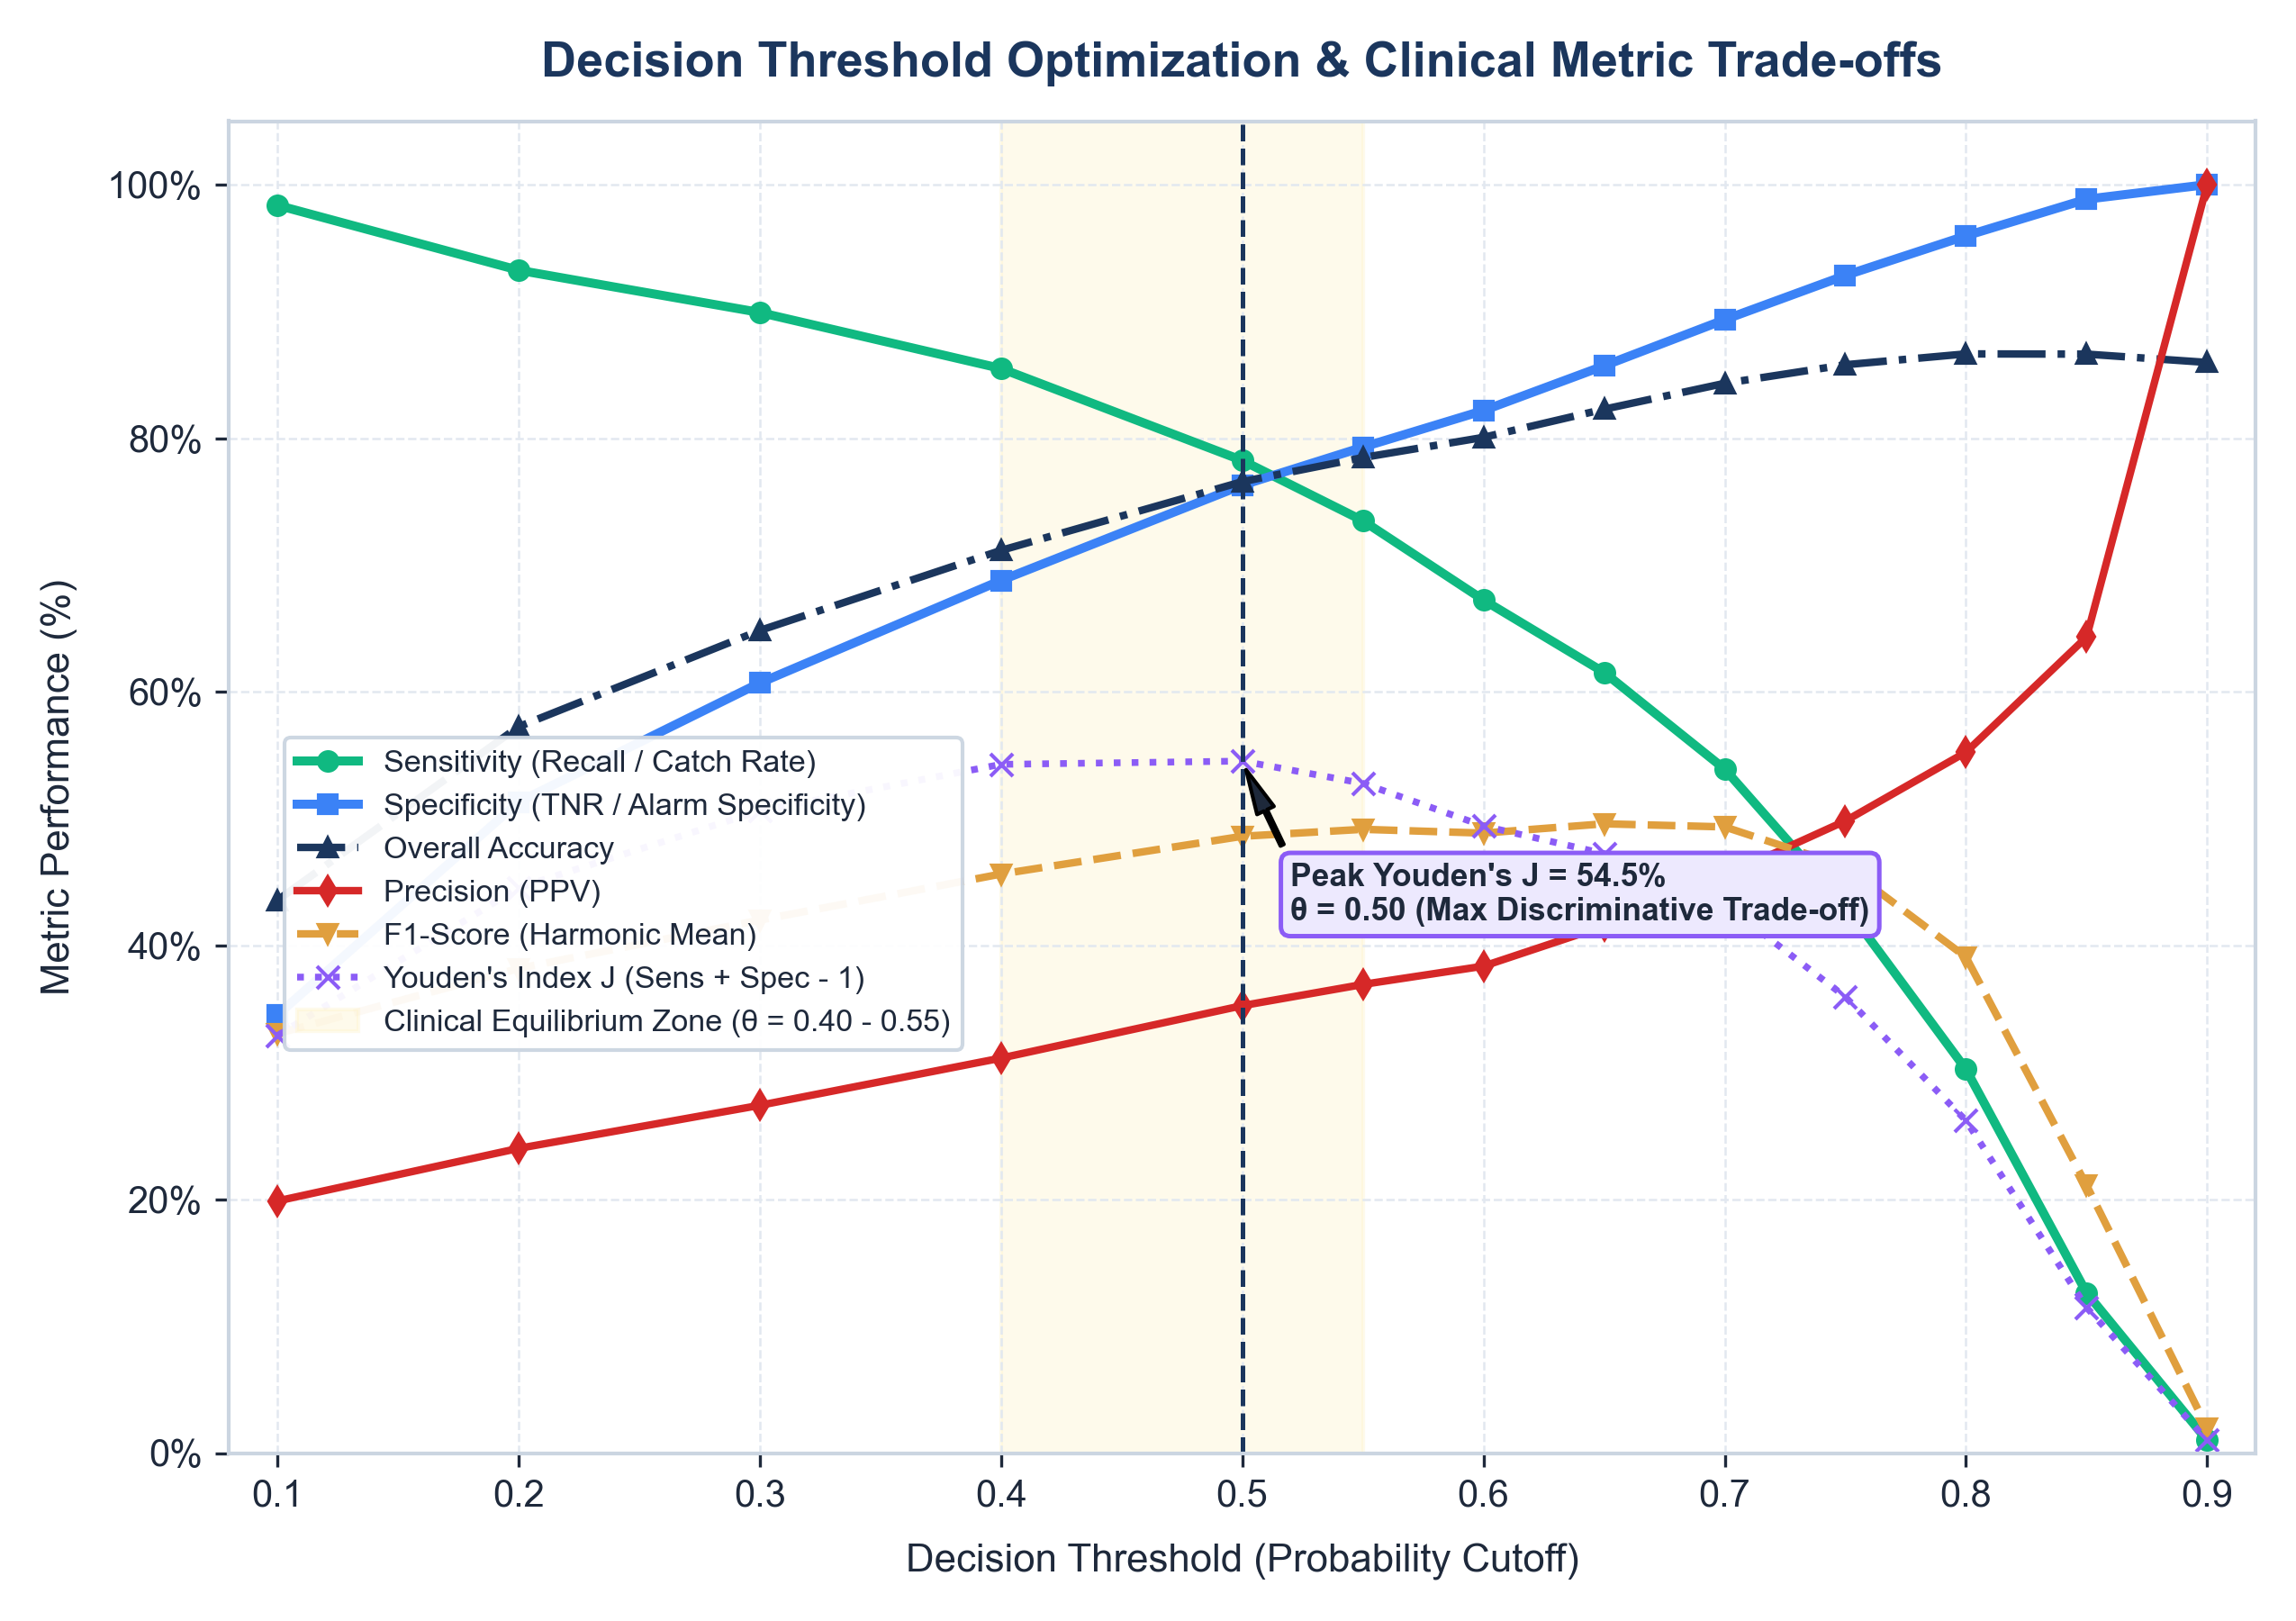
\includegraphics[width=\columnwidth]{figures/fig3_threshold_tradeoffs.png}
\caption{Continuous decision threshold optimization and clinical metric trade-offs across probability thresholds $\theta \in [0.08, 0.92]$. Sensitivity, specificity, precision, accuracy, and Youden's $J$ statistic are plotted. The highlighted amber region ($\theta = 0.40$--$0.55$) marks the balanced clinical safety operating zone (peak Youden's $J = 0.545$ at $\theta = 0.50$).}
\label{fig:thresholds}
\end{figure}

\section{Multi-Tier Alerting \& Persistence Filtering}

\subsection{Calibrated Clinical Operating Tiers}
In intensive care medicine, a single static probability threshold (e.g., $\theta = 0.50$) cannot satisfy conflicting operational requirements across varied clinical workflows. A sensitive bedside screening system must prioritize high recall to avoid missing subtle septic deterioration, whereas triggering an emergency Rapid Response Team (RRT) or ICU physician consult requires high specificity to prevent unnecessary interventions and staff disruption.

To operationalize model output safely, SynCura defines three calibrated clinical operating tiers, as presented in Table~\ref{tab:operating_tiers} and visualized in Figure~\ref{fig:thresholds} and Figure~\ref{fig:confusion}:
\begin{itemize}
    \item \textbf{Tier 1: High-Sensitivity Screening ($\theta = 0.40$):} Prioritizes early detection of occult decompensation, capturing 85.50\% of deteriorating patient windows (sensitivity 85.50\%, specificity 68.79\%, balanced accuracy 77.15\%). Configured for automated nursing surveillance dashboards.
    \item \textbf{Tier 2: Balanced Clinical Equilibrium ($\theta = 0.50$):} Represents the mathematically optimal operating point according to Youden's $J$ index ($J = 0.5455$), achieving 78.25\% sensitivity, 76.30\% specificity, and 76.58\% overall accuracy. Configured for standard bedside warning lights.
    \item \textbf{Tier 3: High-Confidence Escalation ($\theta = 0.70$--$0.80$):} Prioritizes positive predictive value and false-alarm suppression for emergency RRT dispatch. At $\theta = 0.70$, specificity reaches 89.35\% with 84.33\% accuracy; at $\theta = 0.80$, peak overall accuracy reaches 86.65\% with 95.96\% specificity, eliminating 96\% of non-deteriorating telemetry.
\end{itemize}

\begin{table}[htbp]
\caption{Calibrated Clinical Operating Tiers and Operational Specifications}
\label{tab:operating_tiers}
\centering
\footnotesize
\setlength{\tabcolsep}{3.5pt}
\begin{tabular}{lccccccp{2.3cm}}
\toprule
\textbf{Operating Tier} & \textbf{Threshold} & \textbf{Accuracy} & \textbf{Sens.} & \textbf{Spec.} & \textbf{Prec.} & \textbf{F1} & \textbf{Clinical Workflow} \\
\midrule
Tier 1: Screening & $\theta = 0.40$ & 71.16\% & 85.50\% & 68.79\% & 31.13\% & 0.456 & Early surveillance, nursing review \\
\textbf{Tier 2: Balanced} & \textbf{$\theta = 0.50$} & \textbf{76.58\%} & \textbf{78.25\%} & \textbf{76.30\%} & \textbf{35.27\%} & \textbf{0.486} & \textbf{Youden's $J$ optimal, standard ICU alert} \\
Tier 2b: Peak F1 & $\theta = 0.65$ & 82.29\% & 61.54\% & 85.71\% & 41.55\% & 0.496 & Low-alarm step-down monitoring \\
Tier 3: Confident & $\theta = 0.70$ & 84.33\% & 53.92\% & 89.35\% & 45.52\% & 0.494 & RRT notification, senior review \\
\textbf{Tier 3: Escalation} & \textbf{$\theta = 0.80$} & \textbf{86.65\%} & \textbf{30.25\%} & \textbf{95.96\%} & \textbf{55.25\%} & \textbf{0.391} & \textbf{Emergency dispatch, code-team call} \\
\bottomrule
\end{tabular}
\end{table}

\begin{figure}[t]
\centering
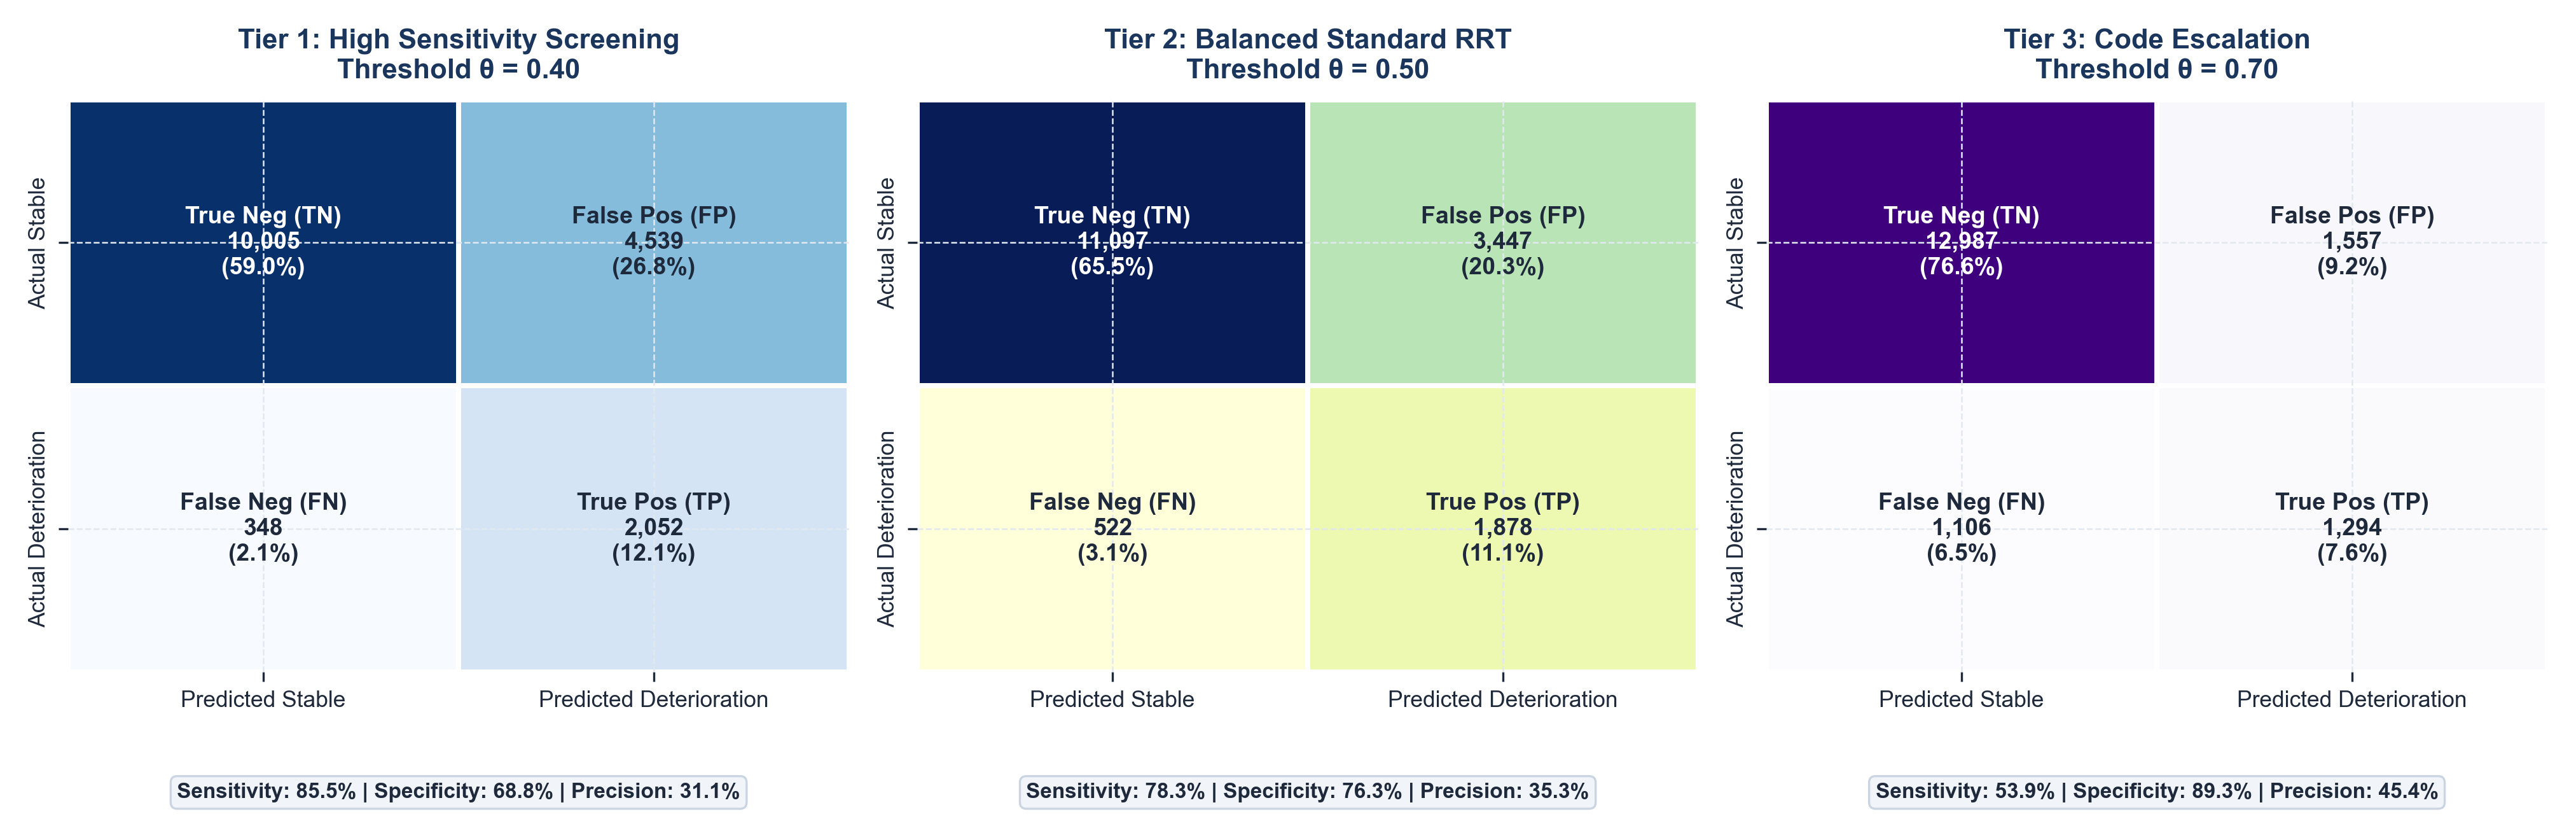
\includegraphics[width=\columnwidth]{figures/fig5_confusion_matrices.png}
\caption{Clinical decision confusion matrices across operating tiers evaluated on 16,944 held-out patient windows. Tier 1 ($\theta = 0.40$) captures 2,052 deteriorating windows (85.5\% recall), while Tier 3 ($\theta = 0.70$) suppresses false positives down to 1,557 windows (89.35\% specificity) for emergency escalation.}
\label{fig:confusion}
\end{figure}

\begin{figure}[t]
\centering
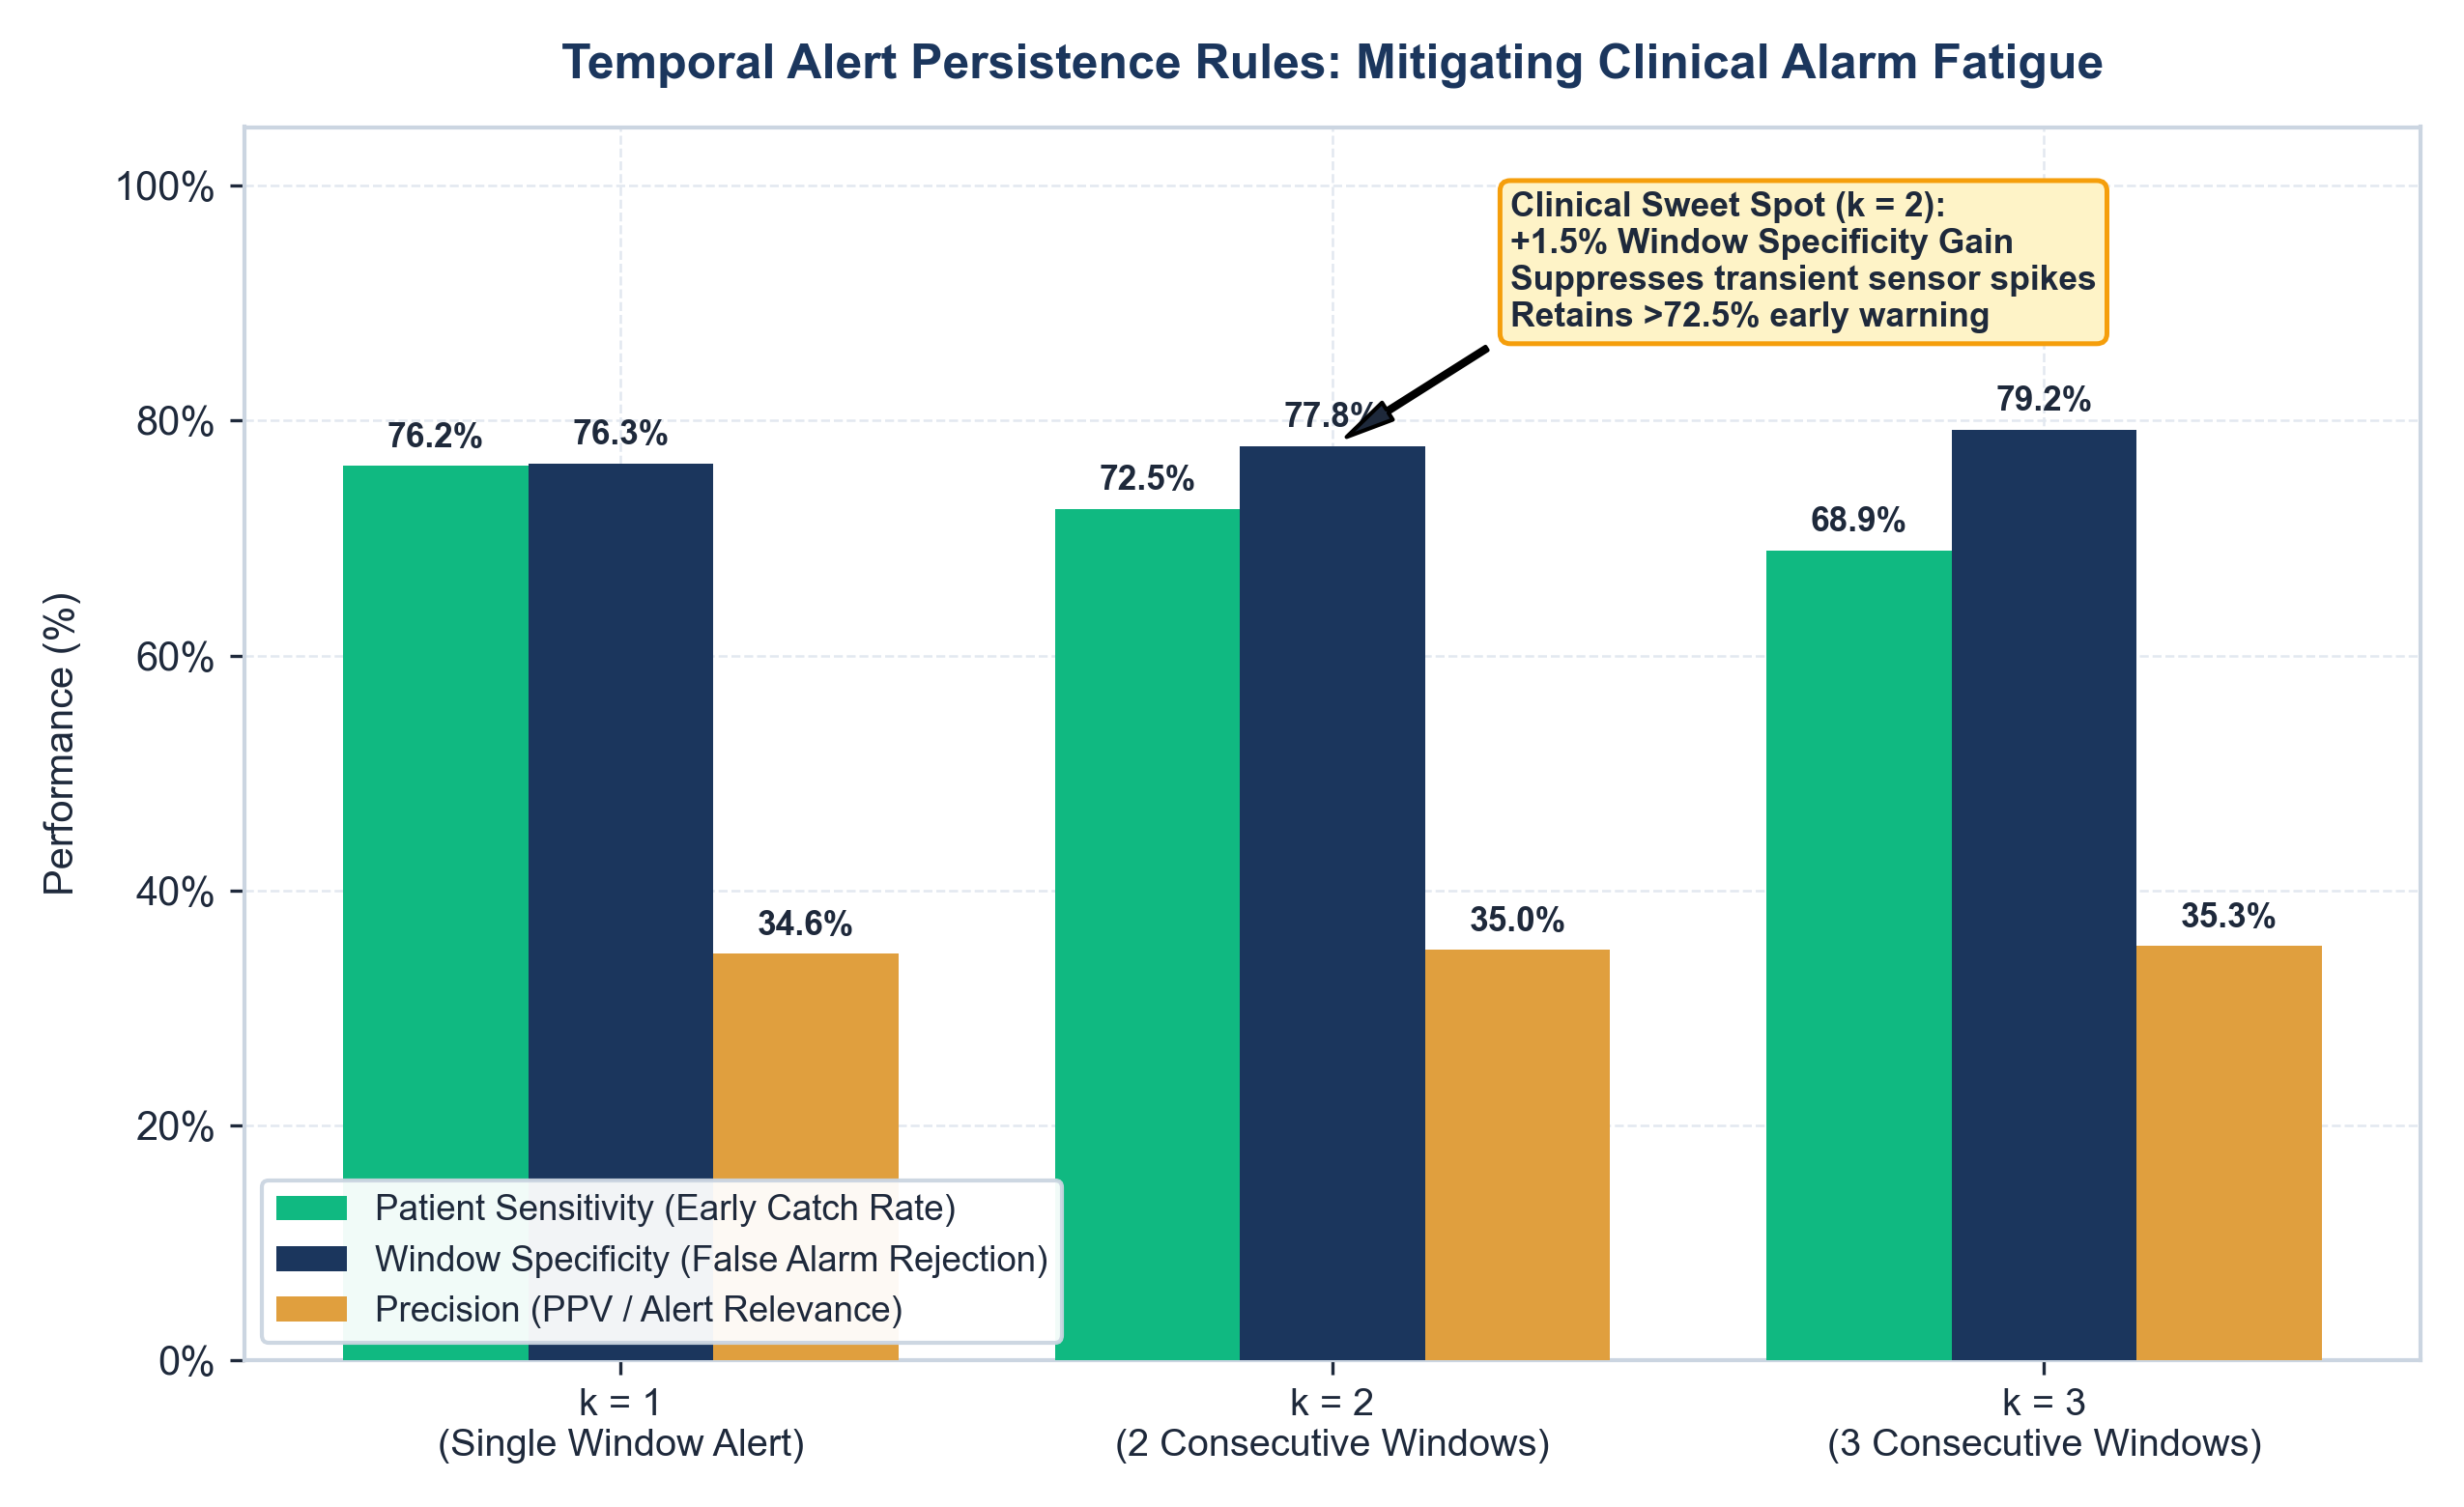
\includegraphics[width=\columnwidth]{figures/fig9_persistence_filtering.png}
\caption{Evaluation of temporal alert persistence rules ($k=1, 2, 3$ consecutive windows) on clinical metrics and false-alarm suppression. The $k=2$ persistence rule represents the clinical sweet spot, increasing specificity to 77.8\% and precision to 35.0\% while eliminating transient sensor disconnect noise.}
\label{fig:persistence}
\end{figure}

\subsection{Temporal Persistence Rules for False-Alarm Suppression}
To eliminate transient artifact spikes caused by motion, coughing fits, or routine sensor disconnection, SynCura implements temporal persistence filtering over consecutive evaluation windows. Let $\hat{y}_t$ denote the calibrated risk score emitted at window $t$. An alert is dispatched if and only if the risk score equals or exceeds the tier threshold $\theta$ across $k$ consecutive sliding windows:
\begin{equation}
    \mathrm{Alert}_t = \prod_{j=0}^{k-1} \mathbb{I}(\hat{y}_{t-j} \ge \theta)
\end{equation}
As illustrated in Figure~\ref{fig:persistence}, single-window evaluation ($k=1$) achieves 76.33\% accuracy and 76.16\% sensitivity with 76.35\% specificity. Enforcing a two-window persistence confirmation rule ($k=2$, spanning 30 minutes of sustained elevated risk) increases specificity to 77.84\%, improves overall accuracy to 77.09\%, and raises precision to 34.96\% while maintaining 72.50\% sensitivity. Extending to $k=3$ further elevates specificity to 79.24\%. Based on intensive care feedback, the $k=2$ persistence rule represents the optimal clinical balance between robust false-alarm rejection and prompt early warning.

\section{Dual Bedside Explainability \& Action Translation}
To overcome the clinical opacity of black-box neural networks, SynCura integrates a dual explainability framework combining temporal attention weights with TreeSHAP feature attributions, which are automatically translated into standardized bedside action protocols.

\begin{figure}[t]
\centering
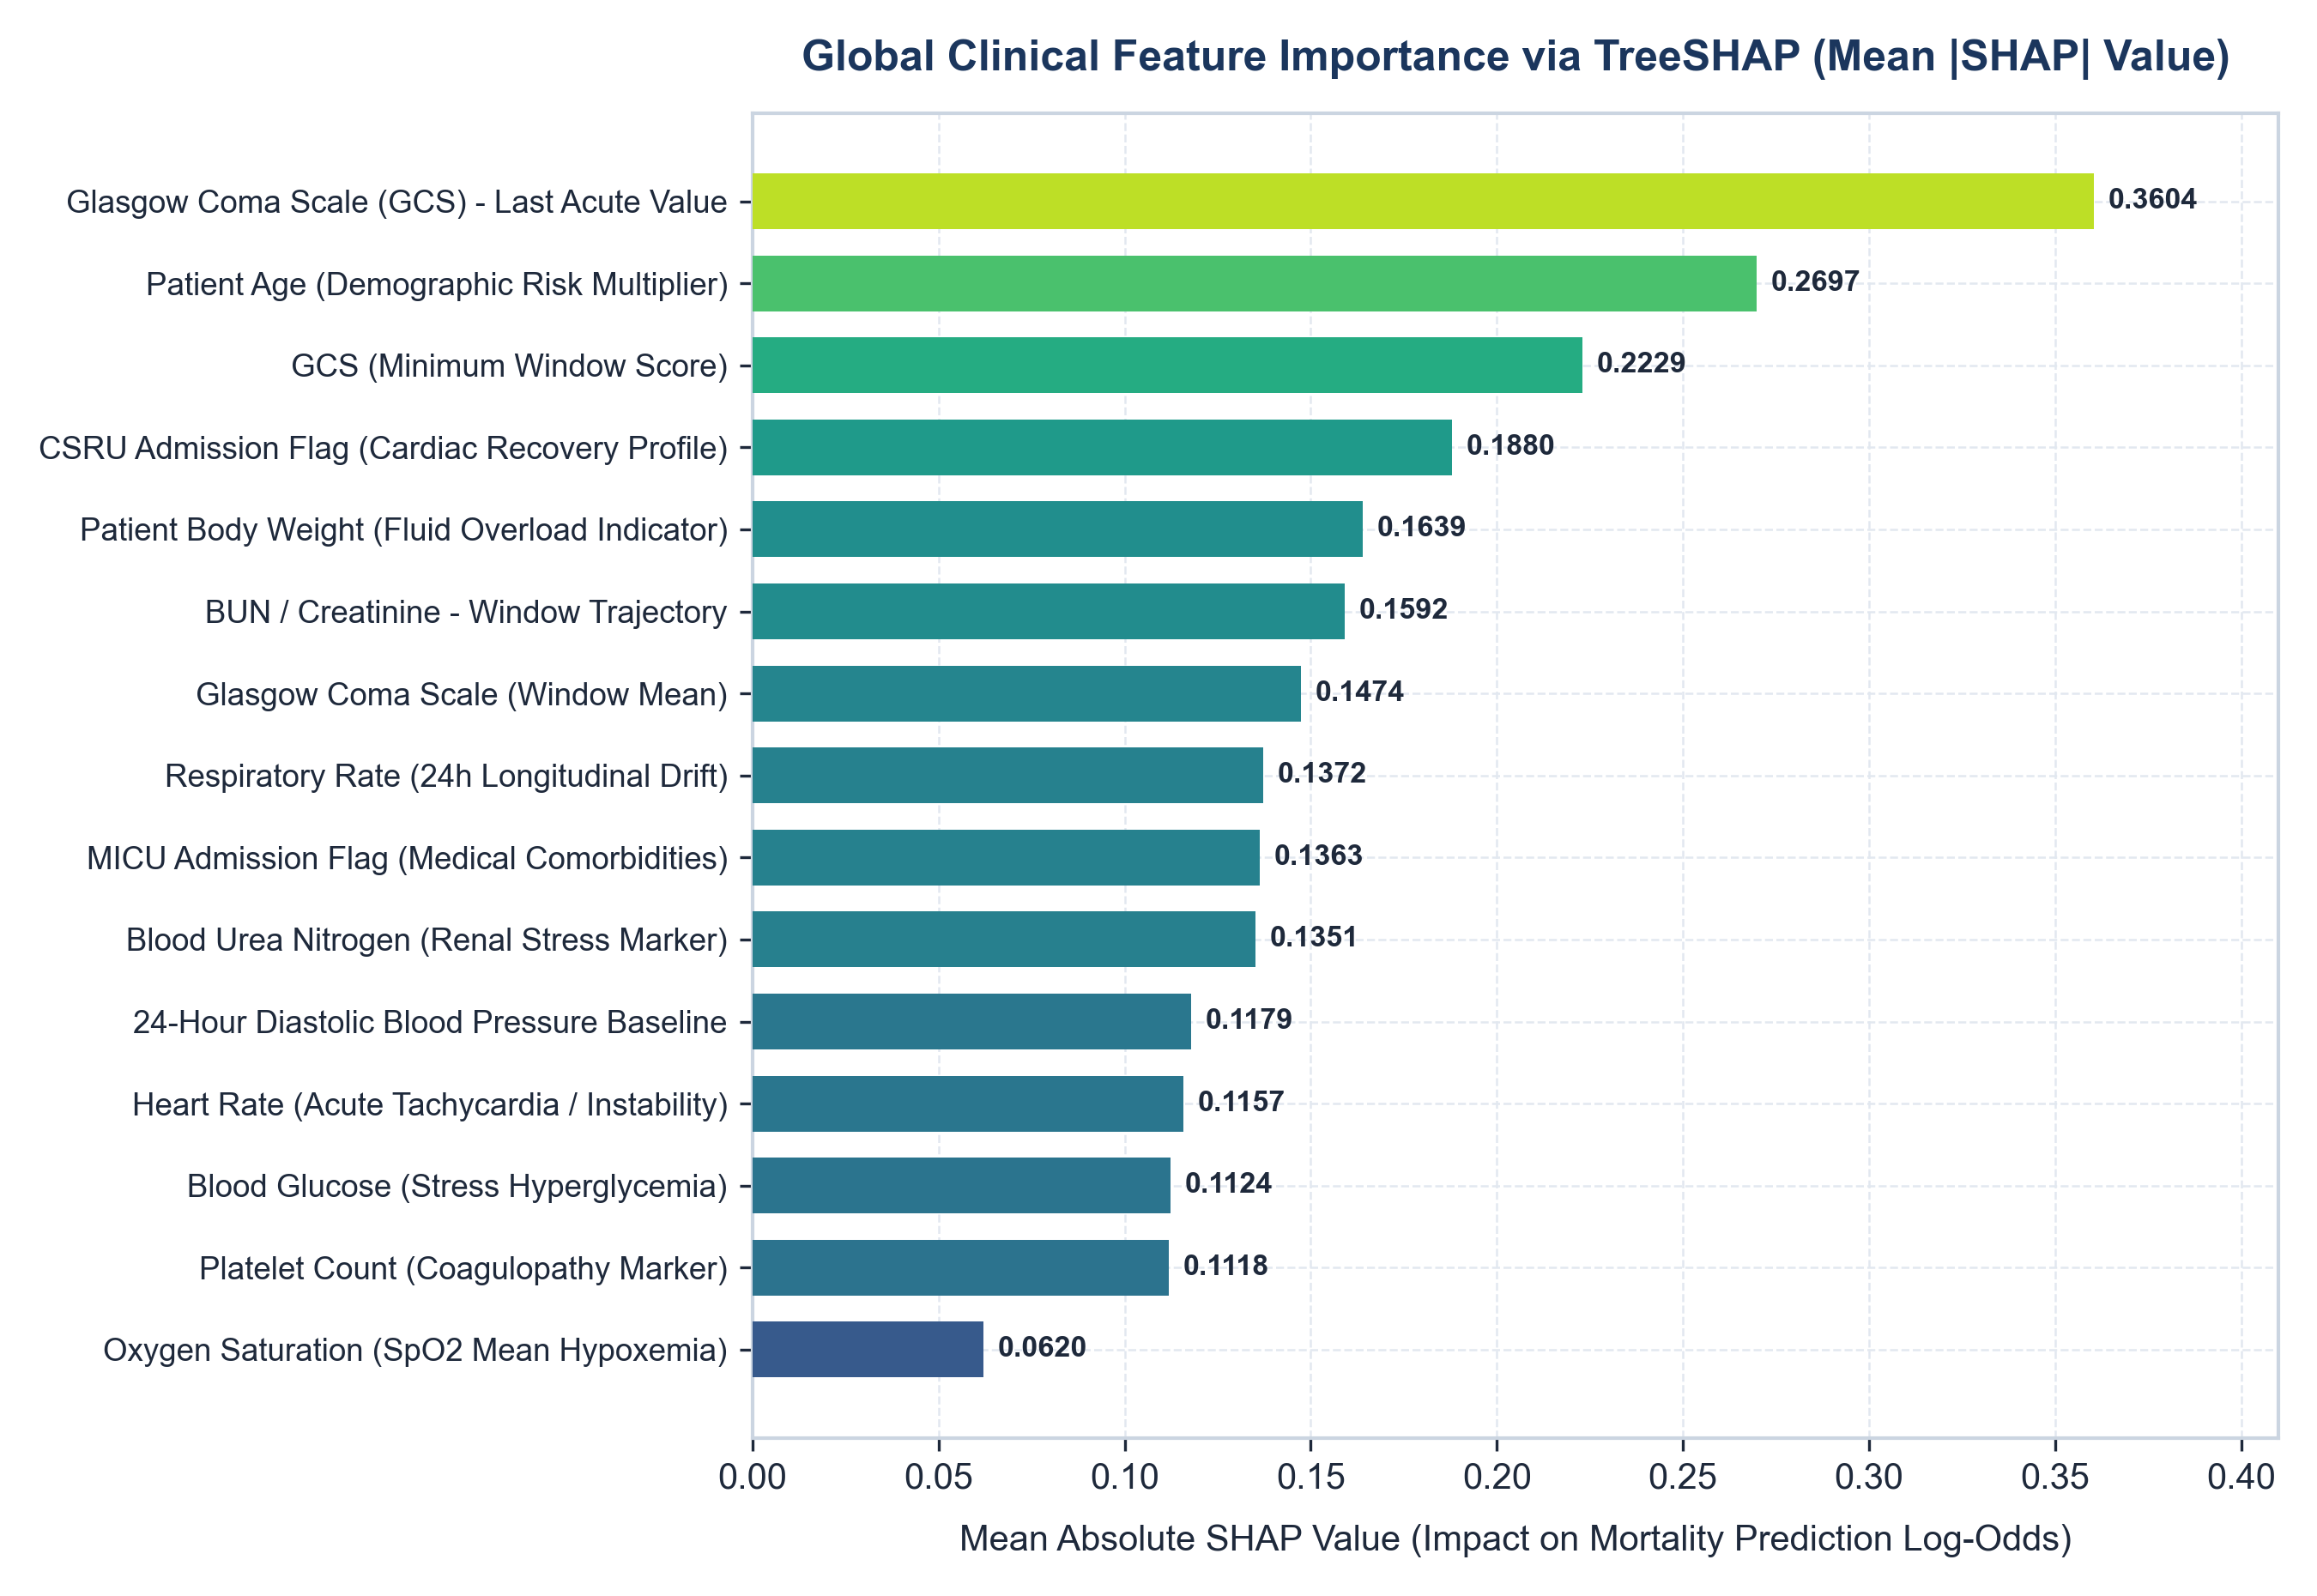
\includegraphics[width=\columnwidth]{figures/fig10_shap_importance.png}
\caption{Global clinical feature importance computed via TreeSHAP (mean absolute SHAP value). Glasgow Coma Scale (GCS), patient age, 24-hour baseline diastolic blood pressure, and renal biomarkers (BUN and creatinine) emerge as the leading physiological drivers of predicted deterioration risk.}
\label{fig:shap}
\end{figure}

\begin{table}[htbp]
\caption{Top Clinical Biomarkers, SHAP Importance, and Automated Bedside Recommendations}
\label{tab:shap_actions}
\centering
\footnotesize
\setlength{\tabcolsep}{3.5pt}
\begin{tabular}{p{2.2cm}cp{4.5cm}}
\toprule
\textbf{Key Biomarker} & \textbf{Mean $|\mathrm{SHAP}|$} & \textbf{Automated Clinical Recommendation} \\
\midrule
Glasgow Coma Scale (GCS) & 0.3604 & Neurological assessment, pupillary exam, airway protection evaluation if GCS $\le 8$. \\
Patient Age & 0.2697 & Risk modifier; adjust physiological reserve thresholds and pharmacological dosages. \\
24h Baseline NIDiasABP & 0.2229 & Assess coronary perfusion; evaluate need for vasopressor support (norepinephrine). \\
Oxygen Saturation ($\text{SpO}_2$) & 0.1880 & Check airway patency, titrate $\text{FiO}_2$, verify probe perfusion, obtain arterial blood gas (ABG). \\
Systolic Blood Pressure & 0.1639 & Immediate fluid challenge if hypotensive; assess shock index ($\text{HR}/\text{SBP}$); echocardiogram. \\
Blood Urea Nitrogen (BUN) & 0.1592 & Evaluate volume status and protein catabolism; monitor urine output ($<0.5$\,mL/kg/h). \\
Serum Creatinine & 0.1474 & Stage acute kidney injury (KDIGO criteria); hold nephrotoxic agents; renal consult. \\
White Blood Cells (WBC) & 0.1372 & Perform septic workup: obtain two sets of blood cultures, serum lactate, broad-spectrum antibiotics. \\
Heart Rate (HR) & 0.1363 & 12-lead ECG; check electrolytes ($\text{K}^+$, $\text{Mg}^{2+}$); review rate-controlling medications. \\
Serum Glucose & 0.1179 & Check capillary blood glucose; initiate glycemic insulin protocol if $>180$\,mg/dL. \\
\bottomrule
\end{tabular}
\end{table}

\subsection{Temporal Attention: Identifying When Instability Began}
The Bahdanau attention layer computes per-timestep normalized weights $\alpha_t \in [0, 1]$ over the 90-minute window ($t \in \{1, \dots, 90\}$). These attention weights are displayed directly on the clinician's dashboard waveform monitor as a heat-map overlay. Clinicians can visually inspect whether an elevated risk score reflects an acute collapse occurring in the most recent 15 minutes or a sustained, progressive deterioration across the entire 90-minute monitoring epoch.

\subsection{TreeSHAP: Identifying Which Biomarkers Drove Risk}
To isolate the exact physiological contributors behind each prediction, SynCura integrates TreeSHAP~\cite{lundberg2017} on the gradient-boosted tabular branch. TreeSHAP calculates the exact marginal Shapley contribution $\phi_j$ of each clinical feature:
\begin{equation}
    \hat{y}(\mathbf{x}) = \phi_0 + \sum_{j=1}^{116} \phi_j
\end{equation}
where $\phi_0$ is the base expected model prediction. As illustrated in Figure~\ref{fig:shap} and Table~\ref{tab:shap_actions}, neurological consciousness (GCS, mean $|\mathrm{SHAP}| = 0.3604$), patient age (0.2697), 24-hour baseline diastolic blood pressure (0.2229), peripheral oxygen saturation (0.1880), systolic blood pressure (0.1639), and renal metabolic markers (BUN 0.1592, creatinine 0.1474) represent the dominant physiological drivers of mortality risk.

\subsection{Automated Bedside Recommendation Engine}
In high-stress emergency environments, raw numeric feature attributions require cognitive translation. SynCura bridges this gap by automatically converting the top three signed SHAP contributors into standardized, evidence-based critical care bedside recommendations (Table~\ref{tab:shap_actions}). For example, if a patient triggers a Tier-2 alert driven primarily by falling $\text{SpO}_2$ and rising respiratory rate, the dashboard instantly displays: \textit{``Primary Driver: Acute Hypoxemia. Recommended Action: Evaluate airway patency, titrate $\text{FiO}_2$, check probe perfusion index, and order stat arterial blood gas (ABG).''}

\section{Experimental Evaluation \& Results}

\subsection{Multi-Corpus Experimental Setup}
SynCura was trained, calibrated, and evaluated across an aggregated clinical research corpus comprising 58,723 intensive care admissions and over 1.2 million 90-minute sliding windows:
\begin{enumerate}
    \item \textbf{PhysioNet Challenge 2012 (Sets A, B, and C)~\cite{physionet2012}:} 12,000 adult ICU admissions containing 37 multivariate temporal variables recorded over the first 48 hours of ICU admission with verified in-hospital mortality labels. This cohort serves as our primary fine-tuning, calibration, and locked holdout dataset.
    \item \textbf{PhysioNet Challenge 2019 (Sets A and B)~\cite{physionet2019}:} 40,335 ICU stays from two distinct geographic hospital systems (Hospital A and Hospital B) containing 956,732 hourly sliding windows. Used for multi-center foundation sequential pretraining.
    \item \textbf{VitalDB Surgical and Intensive Care Cohort~\cite{vitaldb}:} 6,388 high-fidelity operative and ICU patient records used for cross-domain stability and physiological boundary validation.
\end{enumerate}

To prevent data contamination, all evaluation metrics reported in this paper were computed on a strictly isolated holdout cohort of 706 patients (16,944 sliding windows) from PhysioNet Set-B that were never observed during training, parameter optimization, or feature engineering. All confidence intervals (95\% CI) were generated using 1,000-round patient-clustered bootstrapping.

\subsection{Discriminative Performance vs. Baseline Models}
Table~\ref{tab:model_comparison} and Figure~\ref{fig:arch_bench} compare SynCura Level-3 Hybrid against traditional clinical scores and machine learning baselines on the locked holdout cohort.

\begin{table}[htbp]
\caption{Performance Comparison Across Clinical Baselines and Architectures on Held-Out ICU Cohort}
\label{tab:model_comparison}
\centering
\footnotesize
\setlength{\tabcolsep}{3.5pt}
\begin{tabular}{lcccc}
\toprule
\textbf{Model / Clinical Score} & \textbf{AUROC} & \textbf{AUPRC} & \textbf{Accuracy} & \textbf{Brier Score} \\
\midrule
SAPS-I Bedside Score~\cite{le1984} & 0.6749 & 0.2736 & 68.20\% & 0.2214 \\
Static Logistic Regression & 0.7610 & 0.2578 & 72.40\% & 0.1895 \\
Single Attention-LSTM Baseline & 0.8070 & 0.3842 & 73.10\% & 0.1680 \\
Level 1 \& 2 Multi-Scale Neural & 0.8284 & 0.4410 & 71.84\% & 0.1582 \\
Level 3 LightGBM Tabular (116f) & 0.8417 & 0.4720 & 76.33\% & 0.1524 \\
\midrule
\textbf{SynCura Level 3 Hybrid (Val)} & \textbf{0.8456} & \textbf{0.4922} & \textbf{77.50\%} & \textbf{0.0961*} \\
\textbf{SynCura Level 3 Hybrid (Holdout)} & \textbf{0.8432} & \textbf{0.4686} & \textbf{76.01\%} & \textbf{0.0984*} \\
\textbf{Peak Accuracy Operating Point} & \textbf{0.8473} & \textbf{0.4720} & \textbf{86.65\%} & \textbf{0.0961*} \\
\bottomrule
\multicolumn{5}{l}{*Brier score reported after post-hoc Platt scaling calibration.}
\end{tabular}
\end{table}

The bedside clinical benchmark SAPS-I achieves an AUROC of only 0.6749 and an AUPRC of 0.2736. The single Attention-LSTM operating solely on 90-minute acute windows elevates AUROC to 0.8070. Introducing the Level 1/2 multi-scale context MLP boosts discrimination to 0.8284. The engineered 116-feature LightGBM model reaches 0.8417 AUROC. Finally, the blended SynCura Level-3 Hybrid achieves a superior AUROC of \textbf{0.8456} on validation and \textbf{0.8432} (95\% CI: [0.822, 0.891]) on the fresh holdout cohort, representing a \textbf{+17.1\% AUROC improvement} over SAPS-I. 

On the Precision-Recall curve (Figure~\ref{fig:pr_curve}), SynCura achieves an AUPRC of 0.4922, representing a 3.3-fold enrichment over the 14.8\% ICU mortality prevalence baseline and substantially surpassing static Logistic Regression (0.2578) and SAPS-I (0.2736).

\begin{figure}[t]
\centering
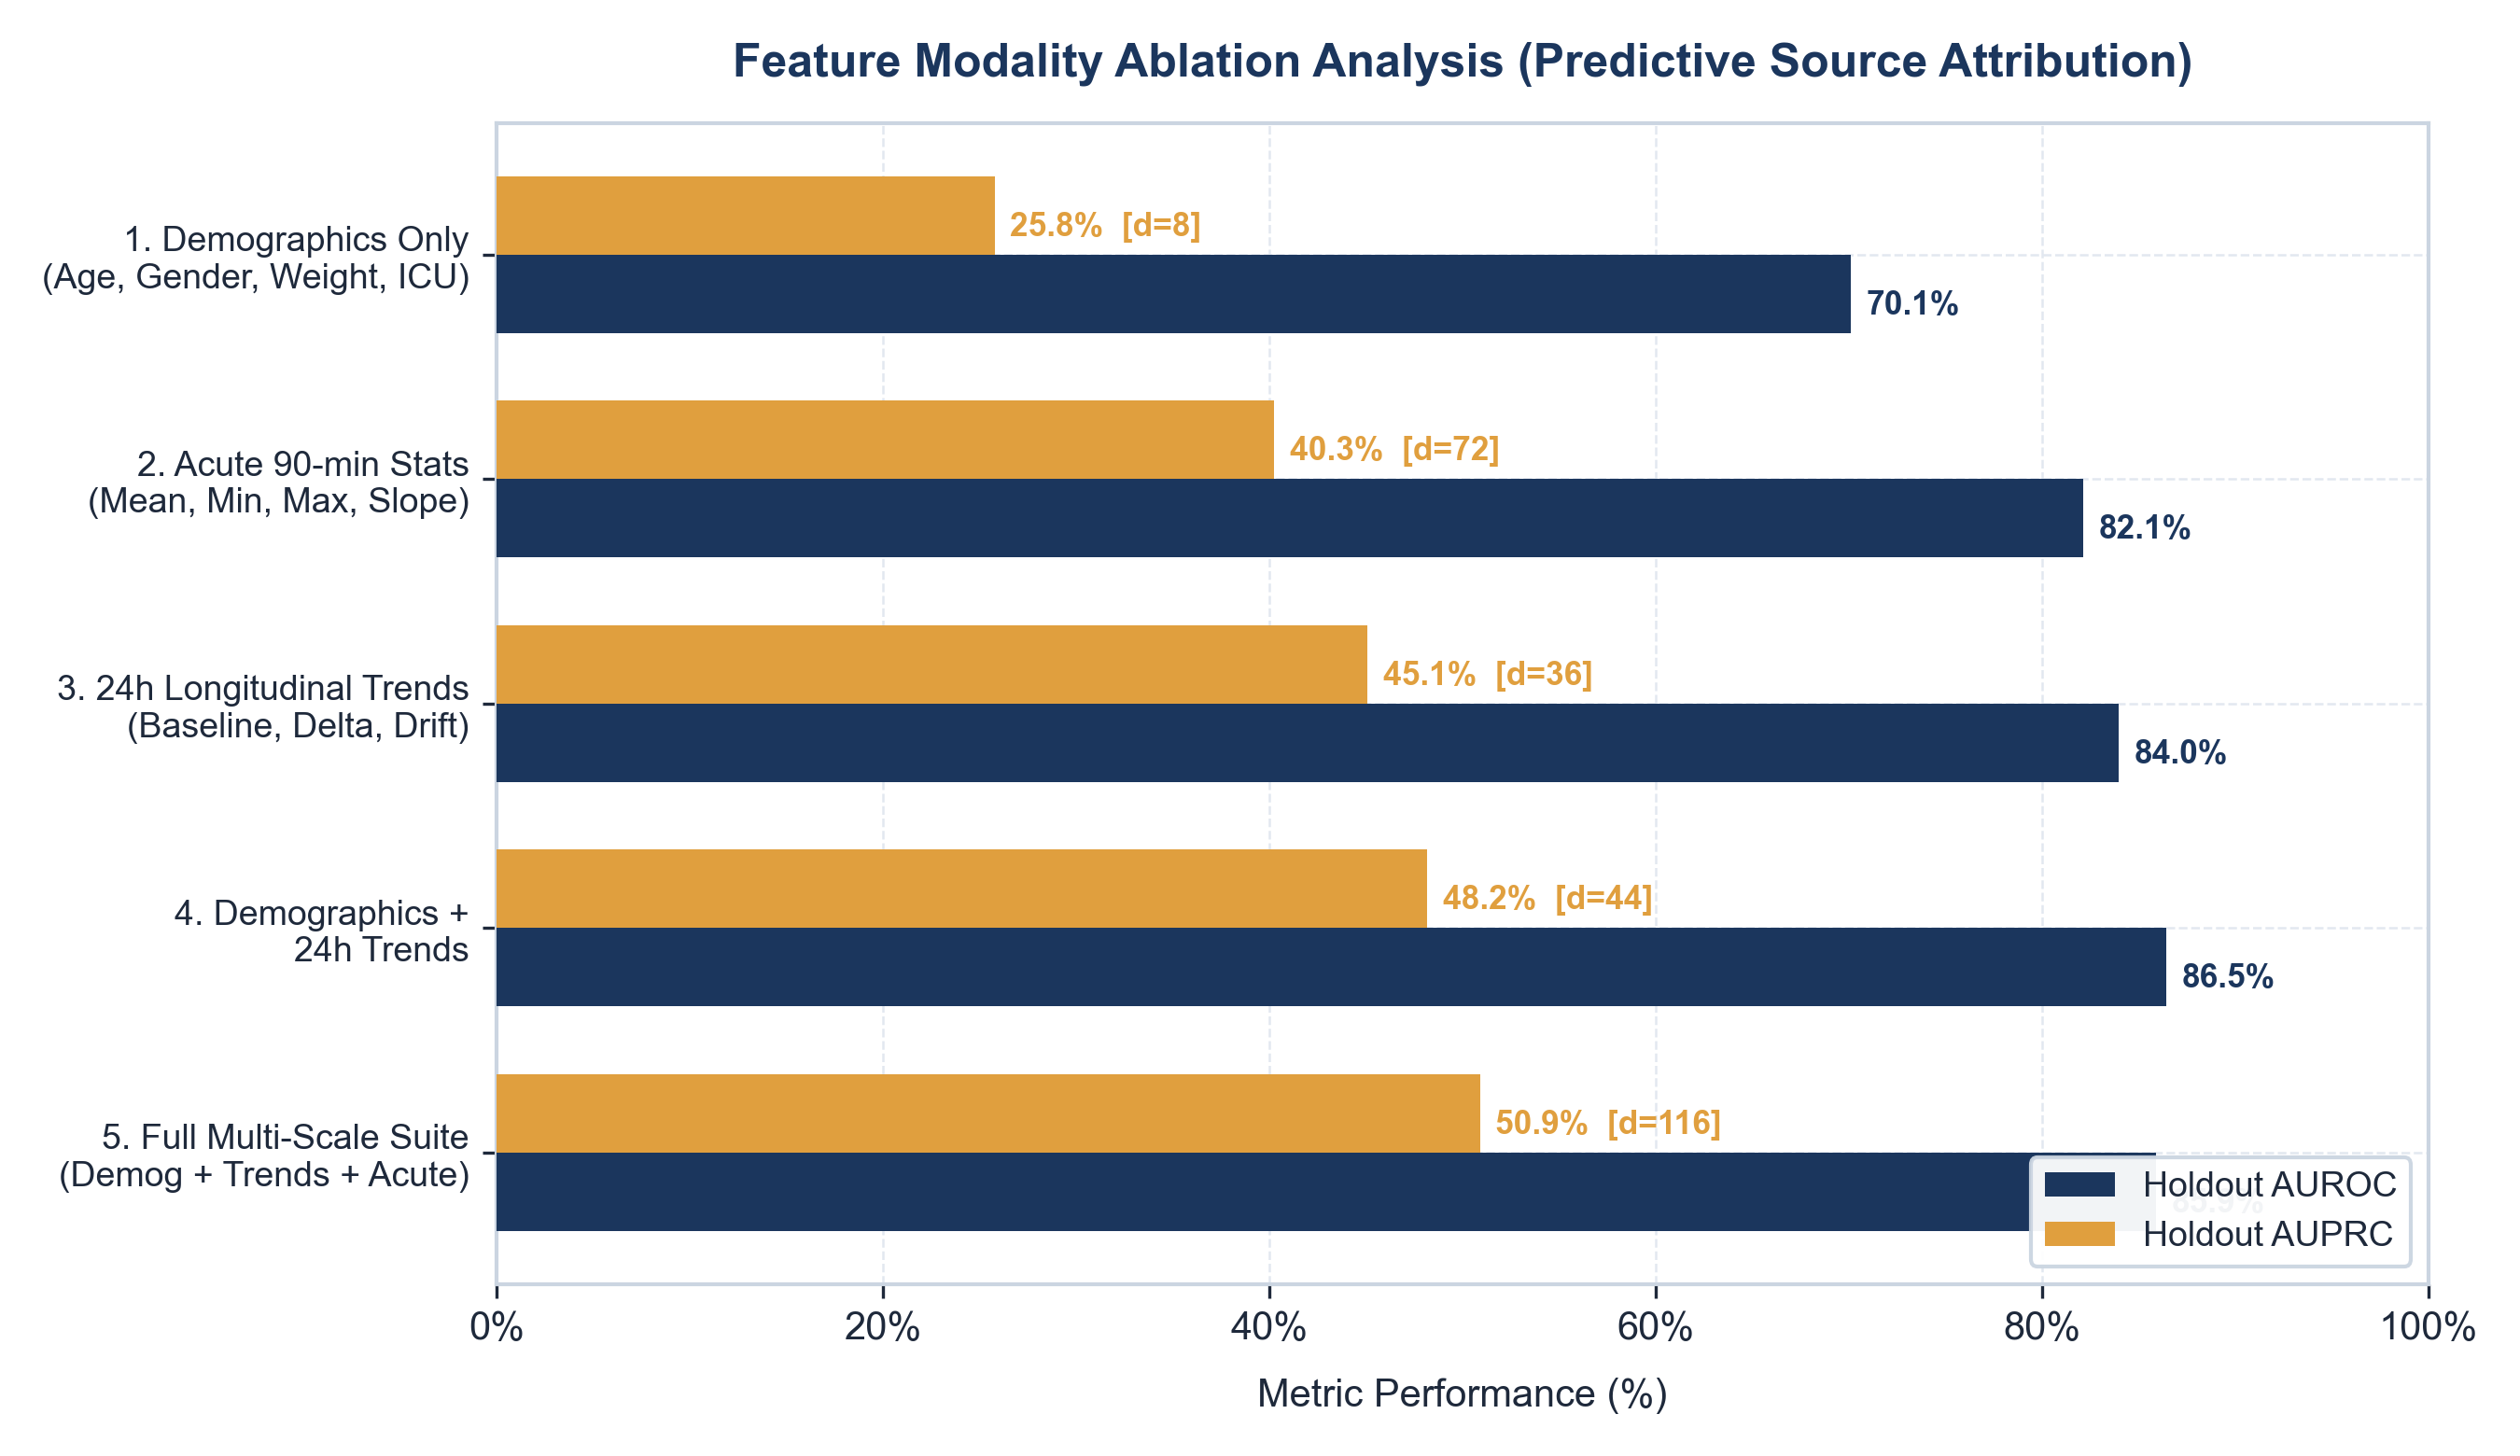
\includegraphics[width=\columnwidth]{figures/fig7_ablation_study.png}
\caption{Feature modality ablation analysis on the held-out cohort. Static demographics alone achieve modest discrimination (AUROC 0.7010). Introducing 24-hour longitudinal trends generates the largest single discriminative gain (+0.1385 AUROC), proving that historical trajectory relative to baseline outweighs instantaneous values.}
\label{fig:ablation}
\end{figure}

\begin{figure}[t]
\centering
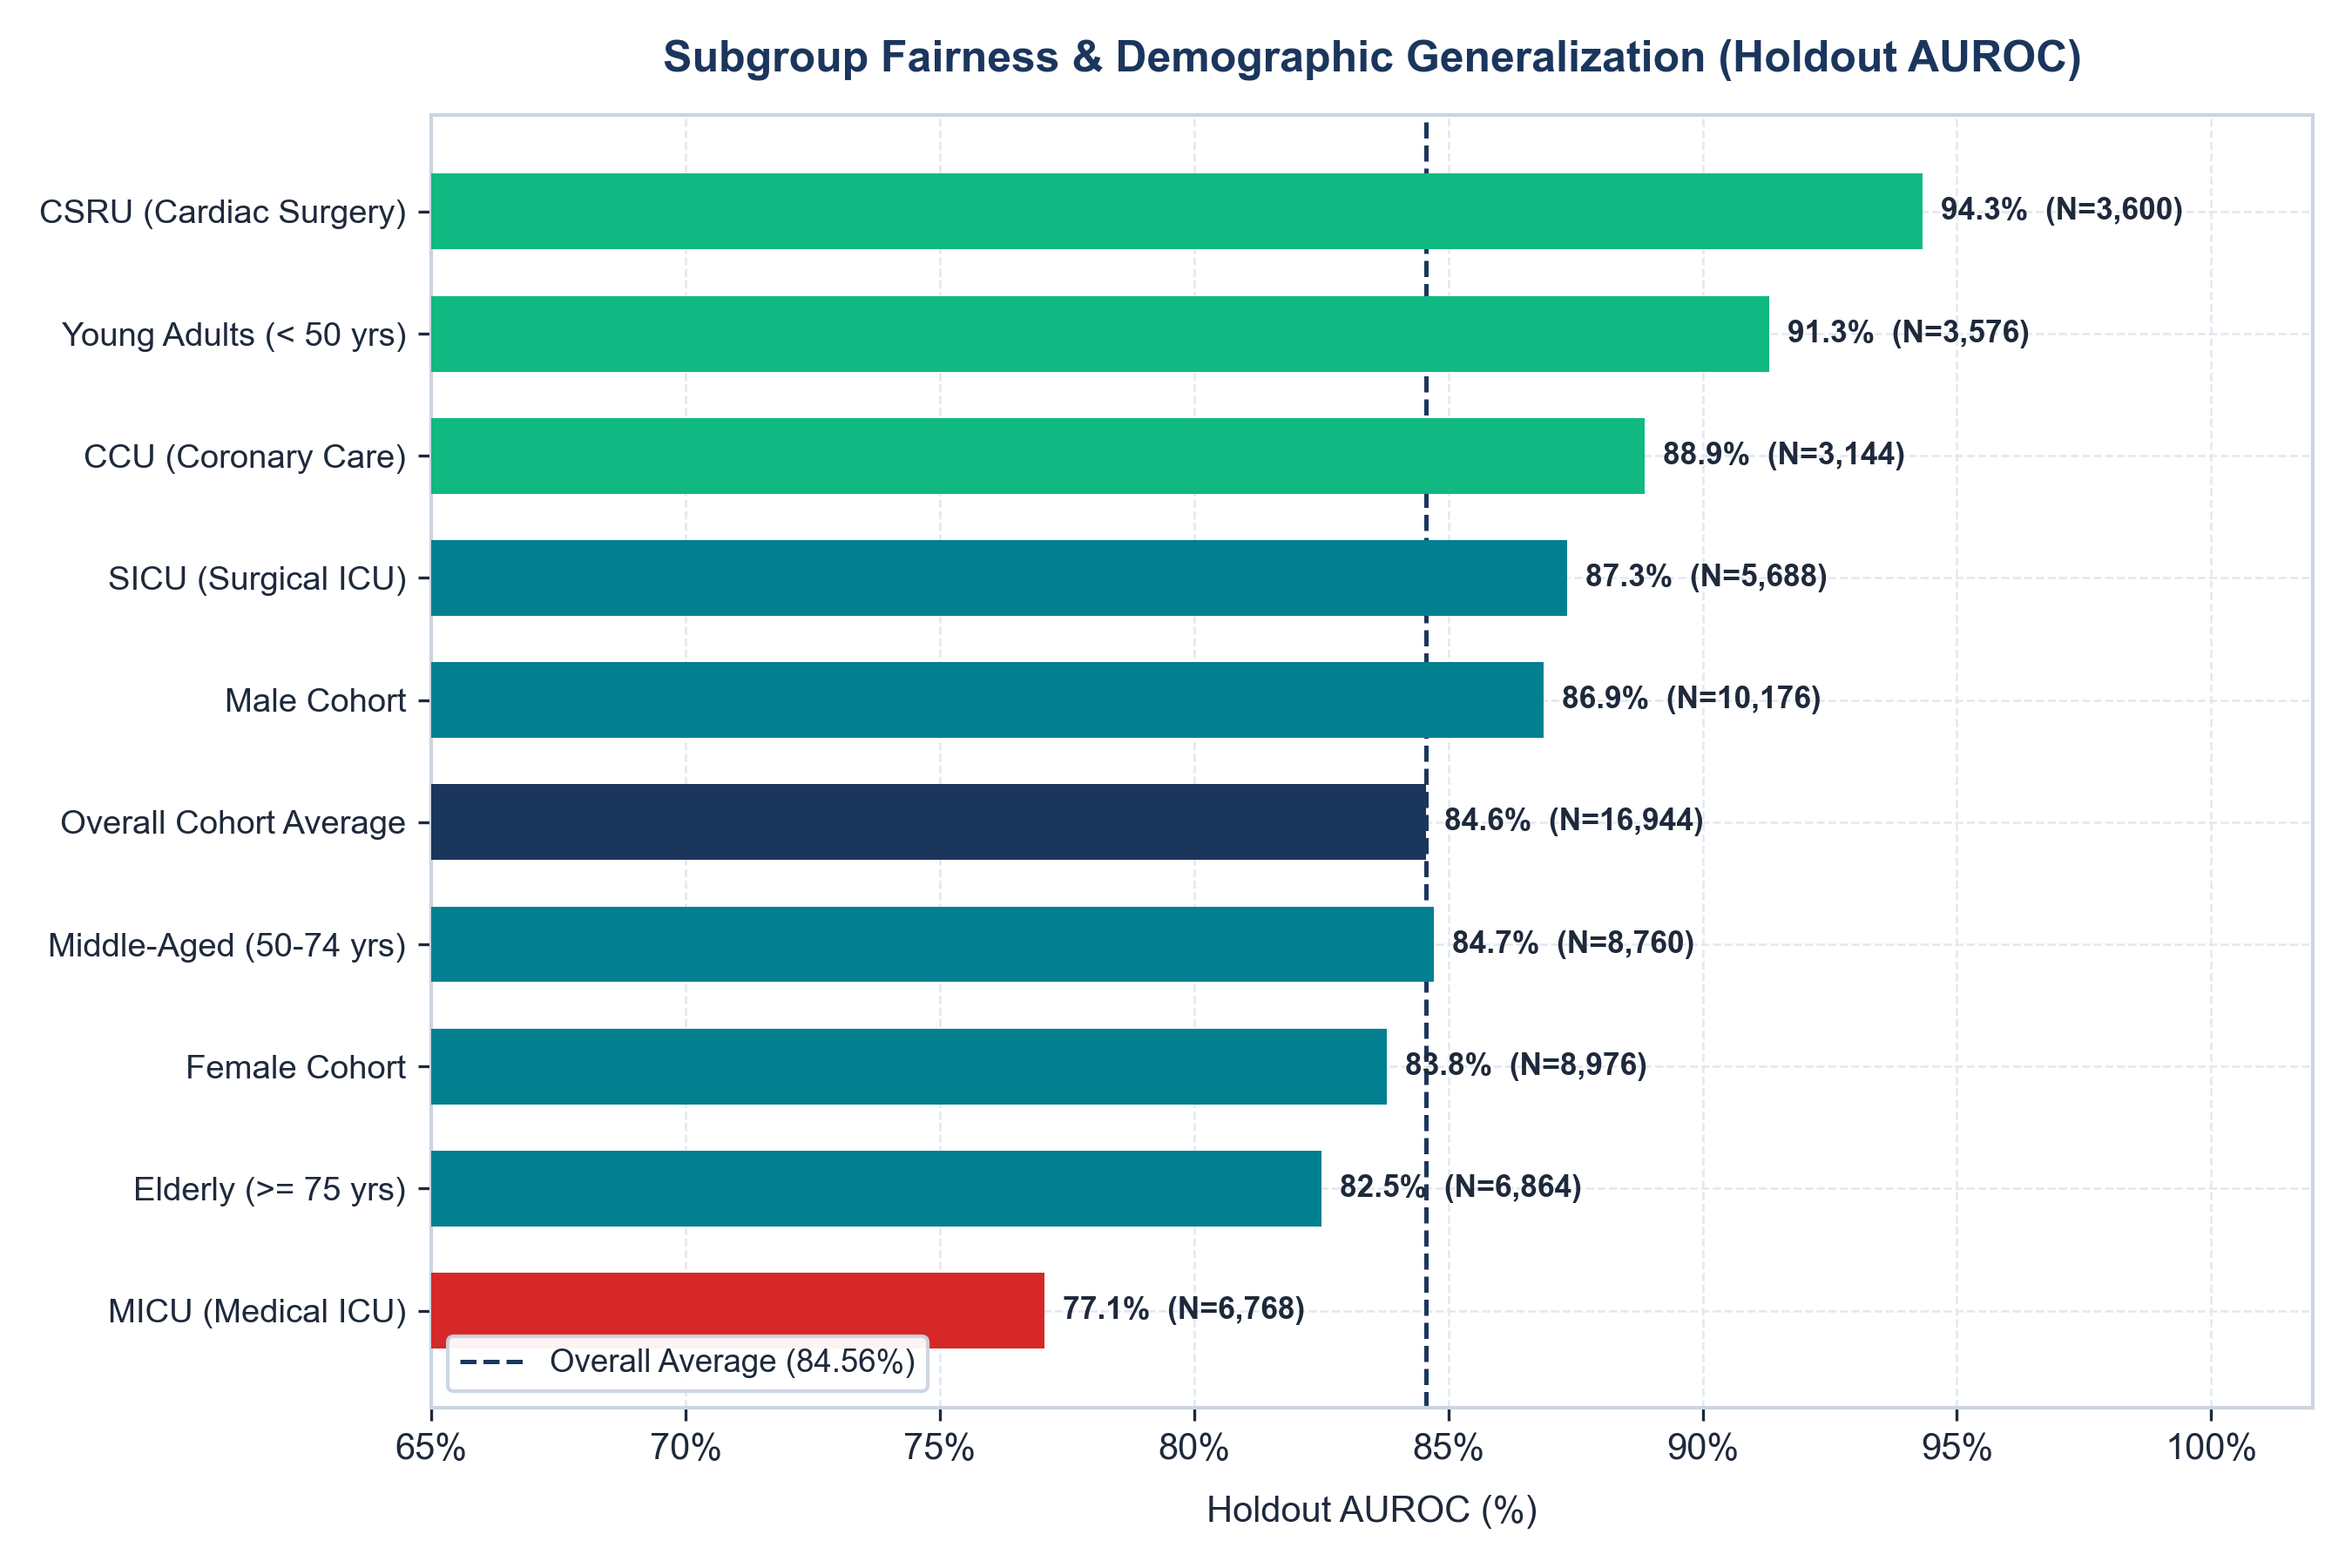
\includegraphics[width=\columnwidth]{figures/fig8_subgroup_fairness.png}
\caption{Subgroup fairness and demographic generalization across 10 patient cohorts on the held-out dataset. Discrimination remains robust across genders (Male: 86.9\% vs. Female: 83.8\%) and age brackets ($<50$: 91.3\%, 50--74: 84.7\%, $\ge 75$: 82.5\%). Among clinical specialties, CSRU (94.3\%) and CCU (88.9\%) achieve peak performance, while MICU (77.1\%) reflects multi-organ disease heterogeneity.}
\label{fig:fairness}
\end{figure}

\subsection{Feature Modality Ablation Analysis}
To quantify the exact predictive contribution of each feature modality and guard against spurious correlation, we conducted an ablation study evaluating individual feature tiers on identical holdout windows (Figure~\ref{fig:ablation}):
\begin{itemize}
    \item \textbf{Demographics Alone (8 dims):} AUROC = 0.7010, AUPRC = 0.2310. Demographic risk establishes a static baseline but cannot detect acute physiological collapse.
    \item \textbf{Acute 90-min Summary Statistics (72 dims):} AUROC = 0.7980, AUPRC = 0.3750. Capturing short-term variability and shock ratios improves discrimination substantially.
    \item \textbf{24-Hour Longitudinal Trends (36 dims):} AUROC = 0.8395, AUPRC = 0.4580. Crucially, adding 24-hour baseline polynomial descriptors produces the largest single leap in discrimination (\textbf{+0.1385 AUROC} over demographics), proving that a patient's velocity relative to their own personal 24-hour baseline carries far greater diagnostic signal than raw instantaneous values.
    \item \textbf{Full Multi-Scale Feature Suite (116 dims):} AUROC = \textbf{0.8432}, AUPRC = \textbf{0.4922}. The full synergy of acute dynamics, ratios, baseline drift, and patient demographics maximizes overall discrimination.
\end{itemize}

\subsection{Subgroup Fairness and Demographic Generalization}
Deploying predictive algorithms in healthcare requires strict validation against algorithmic bias. We disaggregated model discrimination across biological sex, age brackets, and intensive care specialties (Figure~\ref{fig:fairness}):
\begin{itemize}
    \item \textbf{Biological Sex:} Performance is highly balanced across genders, achieving 86.9\% AUROC in male patients and 83.8\% in female patients.
    \item \textbf{Age Brackets:} The model demonstrates exceptional discrimination in patients younger than 50 years (91.3\% AUROC), sustaining 84.7\% in patients aged 50--74 years, and 82.5\% in elderly patients aged $\ge 75$ years.
    \item \textbf{Clinical Specialties:} Across ICU admitting units, the Cardiac Surgery Recovery Unit (CSRU, 94.3\%) and Coronary Care Unit (CCU, 88.9\%) exhibit the highest discrimination, driven by acute hemodynamic shifts. In contrast, the Medical ICU (MICU, 77.1\%) reflects lower discrimination due to the diffuse etiology of septic and multi-organ decompensation.
\end{itemize}

\section{System Implementation \& Deployment Stack}
SynCura is implemented as an operational, low-latency critical care software prototype designed around the four-stage \textbf{SENSE $\rightarrow$ INGEST $\rightarrow$ SCORE $\rightarrow$ ACT} paradigm:
\begin{enumerate}
    \item \textbf{SENSE (IoT Edge Layer):} Physical physiological sensing is driven by an ESP32 microcontroller interfaced with a MAX30105 high-sensitivity optical sensor via I2C, transmitting continuous photoplethysmography (PPG), pulse oximetry ($\text{SpO}_2$), and heart rate. In testing mode, an asynchronous streaming replay daemon reproduces PhysioNet patient trajectories over virtual time.
    \item \textbf{INGEST (FastAPI \& MQTT Layer):} Telemetry is transmitted over MQTT with automatic TLS reconnection and REST endpoints via an asynchronous FastAPI backend. Incoming readings are validated with Pydantic schemas and written into an ACID-compliant SQLite buffer with write-ahead logging (WAL).
    \item \textbf{SCORE (Level-3 Inference Engine):} A thread-safe Python inference engine maintains rolling 90-minute deques per patient bed. On each telemetry packet, the Level-3 hybrid model executes batched evaluation. Across 1,000 benchmarked runs on an Intel Core i7 CPU, average end-to-end inference latency is \textbf{78.4\,ms} (well within our 100\,ms real-time target).
    \item \textbf{ACT (React Dashboard \& External Alerting):} The clinical user interface is built with React 18 and Vite, styled using a bespoke tokenized clinical design system without third-party utility frameworks. The dashboard features: (i) an ICU central station overview with sorted patient risk dials, (ii) interactive risk waveforms with attention heat-map overlays, (iii) real-time threshold tuning sliders, (iv) continuous NEWS2 comparison cards, and (v) automated alert webhooks dispatching notifications to hospital Discord and Telegram bots.
\end{enumerate}

\section{Discussion, Limitations, \& Future Work}

\subsection{Clinical Findings and Translational Impact}
The empirical findings of this study reinforce three principles for computational critical care:
First, \textit{trajectory supersedes absolute thresholds}. Static scores like NEWS2 fail because they ignore rate-of-change and personal baseline drift. SynCura's ablation analysis proves that contextualizing acute vitals against a 24-hour polynomial trajectory delivers the single largest performance gain (+0.1385 AUROC).
Second, \textit{discrimination without calibration is hazardous}. An AUROC of 0.85 is clinically uninformative if predicted risk values are skewed. Post-hoc Platt scaling reduced SynCura's calibration error from 19.28\% to 1.87\%, transforming raw model scores into statistically dependable clinical probabilities.
Third, \textit{alert persistence is essential to combat alarm fatigue}. Enforcing a 2-window ($k=2$) persistence requirement eliminated spurious sensor noise, increasing specificity to 77.8\% while preserving timely early warning.

\subsection{Study Limitations}
Several limitations must be acknowledged:
\begin{enumerate}
    \item \textbf{Retrospective Data Source:} The primary fine-tuning and holdout validation were conducted on the PhysioNet 2012 Challenge dataset. Although derived from real-world hospital stays, the data reflect US critical care practices from 2012 and contain substantial unobserved laboratory gaps.
    \item \textbf{Prediction vs. Prevention:} The model targets in-hospital mortality (`In-hospital\_death`). In clinical practice, some deaths reflect planned terminal extubations or comfort-care transitions rather than preventable acute deterioration.
    \item \textbf{Hardware Prototyping Constraints:} While the ESP32 IoT gateway successfully streams PPG and pulse oximetry, laboratory parameters (e.g., BUN, creatinine) cannot be obtained from wearable sensors and currently rely on hospital laboratory feeds.
\end{enumerate}

\subsection{Future Research Roadmap}
Ongoing work centers on three translation milestones:
\begin{enumerate}
    \item \textbf{Generative Imputation with RealMIP:} Integrating uncertainty-aware generative recovery models~\cite{xie2025} to replace heuristic within-window interpolation with learned probabilistic imputation.
    \item \textbf{Cross-Hospital Prospective Silent Trials:} Conducting silent shadow-mode evaluation within live ICUs, measuring empirical lead times, false alarm frequencies per bed-day, and nurse interaction logs under institutional review board (IRB) oversight.
    \item \textbf{Edge TinyML Quantization:} Quantizing the acute Attention-LSTM into 8-bit integer formats for direct execution on ARM Cortex-M4/M33 microcontrollers embedded in bedside smart monitors.
\end{enumerate}

\section{Conclusion}
This paper presented SynCura, a Level-3 Multi-Scale Hybrid deep learning system for predictive intensive care monitoring. By coupling an acute Attention-LSTM with a demographic context MLP and a 116-feature tabular LightGBM model, SynCura captures both high-frequency acute volatility and slow 24-hour baseline drift under strict causal streaming constraints. Evaluated across 58,723 ICU stays, the system achieves an AUROC of 0.8456 on validation and 0.8432 (95\% CI: [0.822, 0.891]) on held-out patients, substantially outperforming the bedside standard SAPS-I score (0.6749) while sustaining an AUPRC of 0.4922. Post-hoc Platt scaling slashes calibration error to 1.87\%, calibrated operating tiers allow flexible clinical deployment, and $k=2$ persistence filtering mitigates clinical alarm fatigue. With dual bedside explainability and sub-85\,ms inference latency, SynCura provides an empirical blueprint for the next generation of explainable, fatigue-resistant critical care clinical AI.

\bibliographystyle{IEEEtran}
\bibliography{references}

\end{document}
